\documentclass[openany,12pt]{book}

% A5 for mobile readability but with balanced margins
\usepackage[a5paper,top=1.2cm, bottom=1.8cm, left=1.5cm, right=1.5cm]{geometry}
\raggedbottom

% Paragraph style: relaxed reading
\setlength{\parindent}{0pt}
\setlength{\parskip}{4pt}

% Colors
\usepackage{xcolor}

% Hyperlinks
\usepackage[unicode, pdftex, colorlinks=true, linkcolor=black, urlcolor=blue]{hyperref}

% Section/chapter formatting
\usepackage{titlesec}

\titleformat{\chapter}[display]
  {\normalfont\Large\bfseries\color{black}}
  {\chaptertitlename\ \thechapter}{14pt}{\LARGE}
\titlespacing*{\chapter}{0pt}{10pt}{12pt}

\titleformat{\section}[hang]
  {\normalfont\Large\bfseries\color{black}}
  {\thesection}{1em}{}
\titlespacing*{\section}{0pt}{8pt}{6pt}

\titleformat{\subsection}[hang]
  {\normalfont\large\bfseries\color{black}}
  {\thesubsection}{1em}{}
\titlespacing*{\subsection}{0pt}{6pt}{4pt}

% Fonts: programmer-friendly
\usepackage[scaled=0.9]{zi4} % Inconsolata

% Listings
\usepackage{listings}
% Define colors
\definecolor{codegray}{rgb}{0.5,0.5,0.5}
\definecolor{codepurple}{rgb}{0.58,0,0.82}
\definecolor{backcolour}{rgb}{0.95,0.95,0.95}
\definecolor{greencolour}{RGB}{0,128,0}

% Define C# style
\lstdefinestyle{csharp}{
  language=[Sharp]C,              % enable C# keywords
  backgroundcolor=\color{black!5},
  commentstyle=\color{greencolour}\ttfamily,
  keywordstyle=\color{blue},
  stringstyle=\color{codepurple},
  basicstyle=\footnotesize\ttfamily,
  breaklines=true,
  tabsize=2,
  showspaces=false,
  showstringspaces=false,
  aboveskip=4pt,                     % less vertical spacing before code
  belowskip=4pt,                     % less vertical spacing after code
  frame=none,
  numbers=none,
  captionpos=b
}

% Math & figures
\usepackage{amsmath}
\usepackage{graphicx}
\usepackage{tikz}
\usetikzlibrary{shapes.geometric, arrows.meta, positioning}
\usetikzlibrary{shadows}
\begin{document}
\title{
    \textcolor{black}{SLANG4.NET} \\[6pt]
    \Large \textnormal{\textcolor{black}{The art of compiler construction using C\#}}
}
\author{Praseed Pai K. T. \\\\[6pt] Version 0.1 Revised for Mobile}
\date{August 2025}
\maketitle

\tableofcontents
\newpage

\mainmatter
\chapter{Abstract Syntax Tree}
\section{Introduction}
Thanks to the availability of information and better tools writing a compiler has become just an excersise in software engineering. The compilers are not difficult programs to write. The various phases of compilers are easy to understand in an independent manner. The relationship is not purely sequential. It takes some time to put phases in perspective in the job of compilation of programs. 
\section{Compiler Phases}
The task of writing a compiler can be viewed in a top down fashion as shown in the diagram. Lexical analysis and parsing go together. AST stands for Abstract Syntax Tree. By walking the tree we can generate code or do interpretation.\\
\tikzset{
  block/.style = {rectangle, draw, text width=4cm, align=center, minimum height=1cm},
  arrow/.style = {thick,->,>=stealth}
}
\begin{tikzpicture}[node distance=1.5cm and 2cm, scale=0.15]
  \node (phase1) [block] {Lexical Analysis};      
  \node (phase2) [block, right=of phase1] {Parsing};
  \node (phase3) [block, below=of phase2] {AST Creation};
  \node (phase4) [block, left=of phase3] {Code generation or Interpretaion};
  \draw [arrow] (phase1) -- (phase2);
  \draw [arrow] (phase2) -- (phase3);
  \draw [arrow] (phase3) -- (phase4);
 \end{tikzpicture}
 \section{Source code}
 The source code of each chapter in this book and the original book is available at:
 \url{https://github.com/praseedpai/SlangForDotNet}
 
This book is availabe at: 
\url{https://github.com/mmj-the-fighter/slang_for_dot_net_revision}

\clearpage
\section{Abstract Syntax Tree}
In computer science, an abstract syntax tree (AST), or just syntax tree, is a tree representation of the abstract (simplified) syntactic structure of source code written in a certain programming language. Each node of the tree denotes a construct occurring in the source code. The syntax is abstract in the sense that it does not represent every detail that appears in the real syntax. For instance, grouping parentheses is implicit in the tree structure, and a syntactic construct such as if cond then expr may be denoted by a single node with two branches.Most of you might not be aware of the fact that , programming languages are hierarchical in nature. We can model programming language constructs as classes. Trees are a natural data structure to represent
most things hierarchical. As a case in the point , let us look a simple expression evaluator . The expression evaluator will support double
precision floating point value as the operands.  The Operators supported are addition ( + ) , subtraction (-), multiplication (*) and division. The Object model support Unary operators (+ , - ) as well. We are planning to use a composition model for modeling an expression. In most imperative programming languages , an expression is something which you evaluate for it's value. Where
as statements are something which you executes for it's effect.
\clearpage
\section{Exp class}
Let us define an abstract class for Exp
\lstset{style=csharp}
\begin{lstlisting}
// Abstract for Expression evaluation
abstract class Exp
{
	public abstract double Evaluate(RUNTIME_CONTEXT cont);
}
\end{lstlisting}
\section{Runtime Context class}
For the time being RUNTIME\_CONTEXT is an empty class
\lstset{style=csharp}
\begin{lstlisting}
// One can store the stack frame inside this class
public class RUNTIME_CONTEXT
{
	public RUNTIME_CONTEXT()
	{
	}
}
\end{lstlisting}
\section{Modeling Expression}
Once you have declared the interface and it's parameters, we can create a hierarchy of classes to model an expression.
\begin{verbatim}
	class Exp // Base class for Expression
		class NumericConstant // Numeric Value
		class BinaryExp // Binary Expression
		class UnaryExp // Unary Expression
\end{verbatim}
Take a look at the listing of NumericConstant class
\clearpage
\subsection{NumericConstant class}
\lstset{style=csharp}
\begin{lstlisting}
// one can store number inside this class
public class NumericConstant : Exp
{
   private double _value;
   
   // Construction does not do much, just keeps the
   // value assigned to the private variable
   public NumericConstant(double value)
   {
      _value = value;
   }
   
   // While evaluating a numeric constant, return the _value
   public override double Evaluate(RUNTIME_CONTEXT cont)
   {
    return _value;
   }
}
\end{lstlisting}
Since the class is derived from Exp , it ought to implement the Evaluate method. In the Numeric Constant node , we will store a IEEE 754 double precision value. While evaluating the tree , the node will return the value stored inside the object.
\clearpage
\subsection{Binary Expression}
In a Binary Expression , one will have two Operands ( Which are themselves expressions of arbitary complexity ) and an Operator.
\lstset{style=csharp}
\begin{lstlisting}
// This class supports Binary Operators like + , - , / , *
public class BinaryExp : Exp
{
   private Exp _ex1, _ex2;
   private OPERATOR _op;
   public BinaryExp(Exp a, Exp b, OPERATOR op)
   {
      _ex1 = a;
      _ex2 = b;
      _op = op;
   }

   // While evaluating apply the operator after 
   // evaluating the left and right operands
   public override double Evaluate(RUNTIME_CONTEXT cont)
   {
      switch (_op)
      {
         case OPERATOR.PLUS:
            return _ex1.Evaluate(cont) + _ex2.Evaluate(cont);
         case OPERATOR.MINUS:
            return _ex1.Evaluate(cont) - _ex2.Evaluate(cont);
         case OPERATOR.DIV:
            return _ex1.Evaluate(cont) / _ex2.Evaluate(cont);
         case OPERATOR.MUL:
            return _ex1.Evaluate(cont) * _ex2.Evaluate(cont);
      }
      return Double.NaN;
   }
}
\end{lstlisting}
\clearpage 
\subsection{Unary Expression}
In an unary expression , one will have an Operand ( which can be an expression of arbitary complexity ) and an Operator which can be applied on the Operand.
\lstset{style=csharp}
\begin{lstlisting}
// This class supports Unary Operators like + , - , / , *
public class UnaryExp : Exp
{
   private Exp _ex1;
   private OPERATOR _op;
   public UnaryExp(Exp a, OPERATOR op)
   {
      _ex1 = a;
      _op = op;
   }

   // While evaluating apply the unary operator after 
   // evaluating the operand.
   public override double Evaluate(RUNTIME_CONTEXT cont)
   {
      switch (_op)
      {
         case OPERATOR.PLUS:
            return _ex1.Evaluate(cont);
         case OPERATOR.MINUS:
            return -_ex1.Evaluate(cont);
      }
      return Double.NaN;
   }
}
\end{lstlisting}
\clearpage 
\section{Main}
In the CallSLANG project, we will include the SLANG\_DOT\_NET assembly before composing the expression.
\\
\lstset{style=csharp}
\begin{lstlisting}
using System;
using System.Collections.Generic;
using System.Linq;
using System.Text;
using SLANG_DOT_NET; // include SLANG_DOT_NET assembly
namespace CallSLANG
{
   class Program
   {
      static void Main(string[] args)
      {
         // Abstract Syntax Tree (AST) for 5*10
         Exp e = 
		new BinaryExp(
		new NumericConstant(5),
          new NumericConstant(10),
          OPERATOR.MUL);
         // Evaluate the Expression
         Console.WriteLine(e.Evaluate(null));

         // AST for -( (10 + (30 + 50 ) )
         e = 
         new UnaryExp(
            	new BinaryExp(new NumericConstant(10),
	          	new BinaryExp(new NumericConstant(30),
            		new NumericConstant(50),
               	OPERATOR.PLUS),
            	OPERATOR.PLUS),
		OPERATOR.MINUS);
         // Evaluate the Expression
         Console.WriteLine(e.Evaluate(null));

         // Pause for a key stroke
         Console.Read();
      }
   } 
}
\end{lstlisting}
\clearpage 
\chapter{Expressions}
\section{INPUT Analysis}
Compilers are programs which translate source language to a target language. The Source language can be a language like C,C++ or Lisp. The potential target languages are assembly languages , object code
for the microprocessors like intel x86, itanium or power pc. There are programs which translate java to C++ and Lisp to C. In such case , target language is another programming language. 

Any compiler has to understand the input. Once it has analyzed the input characters , it should convert the input into a form which is suitable for further processing. Any input has to be parsed before the object code translation. 

To Parse means to understand. The Parsing process works as follows
The characters are grouped together to find a token ( or a word ). Some examples of the tokens are'+','*',while , for , if etc. The module which reads character at a time and looks for legal token is called
a lexical analyzer or Lexer. 

The input from the Lexer is passed into a module which identifies whether a group of tokens form a valid expression or a statement in the program. The module which determines the validity of expressions is called a parser. Rather than doing a lexical scan for the entire input , the parser requests the next token from the lexical analyzer. They act as if they are co-routines.

To put everything together let us write a small program which acts a four function calculator. The calculator is capable of evaluating mathematical expressions which contains four basic arithmetical operators, paranthesis to group the expression and unary operators.

Given below is the Lexical Specifications of the calculator.
\lstset{style=csharp}
\begin{lstlisting}
TOK_PLUS: '+'
TOK_MUL: '*'
TOK_SUB: '-'
TOK_DIV: '/'
TOK_OPAREN: '('
TOK_CPAREN: ')'
TOK_DOUBLE: [0-9]+
\end{lstlisting}


The lexical specification we just saw can be converted into C\# as follows:
\lstset{style=csharp}
\begin{lstlisting}
// Enumeration for Tokens
public enum TOKEN {
	ILLEGAL_TOKEN = -1, // Not a Token
	TOK_PLUS = 1, // '+'
	TOK_MUL, // '*'
	TOK_DIV, // '/'
	TOK_SUB, // '-'
	TOK_OPAREN, // '('
	TOK_CPAREN, // ')'
	TOK_DOUBLE, // '('
	TOK_NULL // End of string
}
\end{lstlisting}
\clearpage
The Lexical Analysis Algorithm scans through the input and returns the token associated with the operator. If it has found out a number returns the token associated with the number. There should be another mechanism to retrieve the actual number identified.

Following pseudo code shows the schema of the lexical analyzer
\lstset{style=csharp}
\begin{lstlisting}
while ( there is input ) {
	switch(currentchar) {
		case Operands:
			advance input pointer
			return TOK_XXXX;
		case Number:
			Extract the number( Advance the input )
			return TOK_DOUBLE;
		default:
		error
	}
}
\end{lstlisting}
The following C\# code is a literal translation of the above algorithm.
\lstset{style=csharp}
\begin{lstlisting}
using System;
using System.Collections.Generic;
using System.Linq;
using System.Text;
namespace SLANG_DOT_NET 
{
	// Enumeration for Tokens
	public enum TOKEN
	{
		ILLEGAL_TOKEN = -1, // Not a Token
		TOK_PLUS = 1, // '+'
		TOK_MUL, // '*'
		TOK_DIV, // '/'
		TOK_SUB, // '-'
		TOK_OPAREN, // '('
		TOK_CPAREN, // ')'
		TOK_DOUBLE, // '('
		TOK_NULL // End of string
	}


	// A naive Lexical analyzer which looks for 
	// operators , Parenthesis and number. 
	// All numbers are treated as IEEE doubles. Only numbers
	// without decimals can be entered. 
	// Feel free to modify the code
	// to accomodate LONG and Double values
	public class Lexer
	{
		String IExpr; // Expression string
		int index; // index into a character
		int length; // Length of the string
		double number; // Last grabbed number from the stream
		
		public Lexer(String Expr)
		{
			IExpr = Expr;
			length = IExpr.Length;
			index = 0;
		}

		// Grab the next token from the stream
		public TOKEN GetToken()
		{
			TOKEN tok = TOKEN.ILLEGAL_TOKEN;
			// Skip the white space
			while (index < length &&
				(IExpr[index] == ' ' || 
				IExpr[index] == '\t')) {
				index++;
			}
			// End of string ? return NULL;
			if (index == length) {
				return TOKEN.TOK_NULL;
			}

			switch (IExpr[index])
			{
				case '+':
				tok = TOKEN.TOK_PLUS;
				index++;
				break;
				
				case '-':
				tok = TOKEN.TOK_SUB;
				index++;
				break;
				
				case '/':
				tok = TOKEN.TOK_DIV;
				index++;
				break;
				
				case '*':
				tok = TOKEN.TOK_MUL;
				index++;
				break;
				
				case '(':
				tok = TOKEN.TOK_OPAREN;
				index++;
				break;
				
				case ')':
				tok = TOKEN.TOK_CPAREN;
				index++;
				break;
				
				case '0':
				case '1':
				case '2':
				case '3':
				case '4':
				case '5':
				case '6':
				case '7':
				case '8':
				case '9':
				{
					String str = "";
					while (index < length &&
					(IExpr[index] == '0' ||
					IExpr[index] == '1' ||
					IExpr[index] == '2' ||
					IExpr[index] == '3' ||
					IExpr[index] == '4' ||
					IExpr[index] == '5' ||
					IExpr[index] == '6' ||
					IExpr[index] == '7' ||
					IExpr[index] == '8' ||
					IExpr[index] == '9'))
					{
						str += 
							Convert.ToString(IExpr[index]);
						index++;
					}
					number = Convert.ToDouble(str);
					tok = TOKEN.TOK_DOUBLE;
				}
				break;
				
				default:
				Console.WriteLine("Error While Analyzing Tokens");
				throw new Exception();
			}
			return tok;
		}
		
		public double GetNumber() { return number; }
	}
}
\end{lstlisting}

\section{The Grammar}
In computer science, a formal grammar (or grammar) is a set of formation rules (grammar) that describe which strings formed from the alphabet of a formal language are syntactically valid within the language. A grammar only addresses the location and manipulation of the strings of the language. It does not describe anything else about a language, such as its semantics (i.e. what the strings mean).

A context-free grammar is a grammar in which the left-hand side of each production rule consists of only a single nonterminal symbol. This restriction is non-trivial; not all languages can be generated by context-free grammars. Those that can are called context-free languages.

The Backus Naur Form (BNF) notation is used to specify grammars for programming languages, commnd line tools, file formats to name a few . The semantics of BNF is beyond the scope of this book.

\subsection{Grammar of the expression evaluator}
\lstset{style=csharp}
\begin{lstlisting}
<Expr> ::= <Term> | <Term> { + | - } <Expr>
<Term> ::= <Factor> | <Factor> {* | /} <Term>
<Factor>::= <number> | ( <expr> ) | {+ | -} <factor>
\end{lstlisting}
There are two types of tokens in any grammar specifications. They are terminal tokens ( terminals ) or non terminals . In the above grammar , operators and \textless number\textgreater are the terminals.

\textless Expr\textgreater,\textless Term\textgreater,\textless Factor\textgreater are non terminals. Non terminals will have at least one entry on the left side. 


In the following three sections the pesudo code snippets for converting each of our non terminals is shown.
Note that they closely match with production rules we stated.
\section{Conversion of Expression}
\lstset{style=csharp}
\begin{lstlisting}
// <Expr> ::= <Term> { + | - } <Expr>
Void Expr() {
	Term();
	if ( Token == TOK_PLUS || Token == TOK_SUB )
	{
		// Emit instructions
		// and perform semantic operations
		Expr(); // recurse
	}
}
\end{lstlisting}

\section{Conversion of Term}
\lstset{style=csharp}
\begin{lstlisting}
// <Term> ::= <Factor> { * | / } <Term>
Void Term() {
	Factor();
	if ( Token == TOK_MUL || Token == TOK_DIV )
	{
		// Emit instructions
		// and perform semantic operations
		Term(); // recurse
	}
}
\end{lstlisting}

\section{Conversion of Factor}
\lstset{style=csharp}
\begin{lstlisting}
// <Factor> ::= <TOK_DOUBLE> | ( <expr> ) | { + |- } <Factor>
Void Factor() {
	switch(Token) {
		case TOK_DOUBLE:
		// push token to IL operand stack return
		
		case TOK_OPAREN:
		Expr(); //recurse
		// check for closing parenthesis and return

		case UNARYOP:
		Factor(); //recurse
		
		default:
		//Error
	}
}
\end{lstlisting}
\section{RD Parser}
The class RDParser is derived from the Lexer class. By using an algorithm by the name Recursive descent parsing , we will evaluate the expression.A recursive descent parser is a top-down parser built from a set of mutually-recursive procedures where each such procedure usually implements one of the production rules of the grammar. Thus the structure of the resulting program closely mirrors that of the grammar it recognizes.
\lstset{style=csharp}
\begin{lstlisting}
using System;
using System.Collections.Generic;
using System.Linq;
using System.Text;
namespace SLANG_DOT_NET
{
	public class RDParser : Lexer
	{
		TOKEN Current_Token;
		public RDParser(String str)
		: base(str)
		{
		}
		
		public Exp CallExpr()
		{
			Current_Token = GetToken();
			return Expr();
		}
		
		public Exp Expr()
		{
			TOKEN l_token;
			Exp RetValue = Term();
			while (Current_Token == TOKEN.TOK_PLUS 
				|| Current_Token == TOKEN.TOK_SUB)
			{
				l_token = Current_Token;
				Current_Token = GetToken();
				Exp e1 = Expr();
				RetValue = new BinaryExp(RetValue, e1,
				l_token == 
				TOKEN.TOK_PLUS ? 
				OPERATOR.PLUS : OPERATOR.MINUS);
			}
			return RetValue;
		}

		public Exp Term()
		{
			TOKEN l_token;
			Exp RetValue = Factor();
			while (Current_Token == TOKEN.TOK_MUL 
				|| Current_Token == TOKEN.TOK_DIV)
			{
				l_token = Current_Token;
				Current_Token = GetToken();
				Exp e1 = Term();
				RetValue = 
				new BinaryExp(RetValue, e1,
				l_token == 
				TOKEN.TOK_MUL ? 
				OPERATOR.MUL : OPERATOR.DIV);
			}
			return RetValue;
		}

		public Exp Factor()
		{
			TOKEN l_token;
			Exp RetValue = null;
			if (Current_Token == TOKEN.TOK_DOUBLE)
			{
				RetValue = new NumericConstant(GetNumber());
				Current_Token = GetToken();
			}
			else if (Current_Token == TOKEN.TOK_OPAREN)
			{
				Current_Token = GetToken();
				RetValue = Expr(); // Recurse
				if (Current_Token != TOKEN.TOK_CPAREN)
				{
					Console.WriteLine("Missing Closing Parenthesis");
					throw new Exception();
				}
				Current_Token = GetToken();
			}
			else if (Current_Token == TOKEN.TOK_PLUS 
				|| Current_Token == TOKEN.TOK_SUB)
			{
				l_token = Current_Token;
				Current_Token = GetToken();
				RetValue = Factor();
				RetValue = 
				new UnaryExp(RetValue,
				l_token == TOKEN.TOK_PLUS ? 
				OPERATOR.PLUS : OPERATOR.MINUS);
			}
			else
			{
				Console.WriteLine("Illegal Token");
				throw new Exception();
			}
			return RetValue;
		}
	} 	
}
\end{lstlisting}

\section{Builder}
Using the Builder Pattern , we will encapsulate the Parser , Lexer class activities
\lstset{style=csharp}
\begin{lstlisting}
using System;
using System.Collections.Generic;
using System.Linq;
using System.Text;
namespace SLANG_DOT_NET
{
	// Base class for all the Builders
	public class AbstractBuilder
	{
	}

	public class ExpressionBuilder : AbstractBuilder
	{
		public string _expr_string;
		public ExpressionBuilder(string expr)
		{
			_expr_string = expr;
		}
		
		public Exp GetExpression()
		{
			try
			{
				RDParser p = 
				new RDParser(_expr_string);
				return p.CallExpr();
			}
			catch (Exception)
			{
				return null;
			}
		}
	}
}
\end{lstlisting}

\section{Main}
In the CallSLang Project , the expression compiler is invoked as follows
\lstset{style=csharp}
\begin{lstlisting}
using System;
using System.Collections.Generic;
using System.Linq;
using System.Text;
using SLANG_DOT_NET;
namespace CallSLANG
{
	class Program
	{
		static void Main(string[] args)
		{
			ExpressionBuilder b = new ExpressionBuilder("-2*(3+3)");
			Exp e = b.GetExpression();
			Console.WriteLine(e.Evaluate(null));
			Console.Read();
		}
	} 
}
\end{lstlisting}
\chapter{Statements}
The crux of the SLANG4.net can be summed up in two sentences
\begin{verbatim}
1. Expression is what you evaluate for it's value.
2. Statement is what you execute for it's effect (on variables).
\end{verbatim}
The above two maxims can be converted into a computational structure as follows:
\lstset{style=csharp}
\begin{lstlisting}
// Expression is what you evaluate for it's value
public abstract class Exp
{
	public abstract double Evaluate(RUNTIME_CONTEXT cont);
}

// Statement is what you Execute for it's Effect
// on variables or lack of it
public abstract class Stmt
{
	public abstract bool Execute(RUNTIME_CONTEXT con);
}
\end{lstlisting}

\section{Print statement}
Let us implement a Print statement for the SLANG4.net compiler. The basic idea is as follows you add a class to model a statement and since the class has to inherit from the Stmt ( abstract class ), it ought to implement Execute Method.
\lstset{style=csharp}
\begin{lstlisting}
// Implementation of Print Statement
public class PrintStatement : Stmt
{
	// At this point of time, Print will
	// spit the value of an Expression on the screen.
	private Exp _ex;
	
	// Ctor just stores the expression passed as parameter
	public PrintStatement(Exp ex)
	{
		_ex = ex;
	}

	// Execute method Evaluates the expression and
	// spits the value to the console using
	// Console.Write statement.
	public override bool Execute(RUNTIME_CONTEXT con)
	{
		double a = _ex.Evaluate(con);
		Console.Write(a.ToString());
		return true;
	}
}
\end{lstlisting}
\section{PrintLine statement}
Let us add a PrintLine statement as well. PrintLine implementation is not different from Print statement. The only difference is it emits a new line after the expression value.
\lstset{style=csharp}
\begin{lstlisting}
// Implementation of PrintLine Statement
public class PrintLineStatement : Stmt
{
	private Exp _ex;
	public PrintLineStatement(Exp ex)
	{
		_ex = ex;
	}
	
	// Here we are calling Console.WriteLine to emit
	// an additional new line .
	public override bool Execute(RUNTIME_CONTEXT con)
	{
		double a = _ex.Evaluate(con);
		Console.WriteLine(a.ToString());
		return true;
	}
}
\end{lstlisting}

\section{Changes in the Parser}
Once we have created to classes to implement Print and PrintLine statement, we need to modify our
parser (frontend ) to support the statement in the language.\\
\subsection{Changes in the Lexer}
We are going to add few more tokens to support the Statements in the SLANG.\\
\lstset{style=csharp}
\begin{lstlisting}
public enum TOKEN
{
	ILLEGAL_TOKEN = -1, // Not a Token
	TOK_PLUS = 1, // '+'
	TOK_MUL, // '*'
	TOK_DIV, // '/'
	TOK_SUB, // '-'
	TOK_OPAREN, // '('
	TOK_CPAREN, // ')'
	TOK_DOUBLE, // 'number'
	TOK_NULL, // End of string
	TOK_PRINT, // Print Statement
	TOK_PRINTLN, // PrintLine
	TOK_UNQUOTED_STRING,
	TOK_SEMI // ;
}
\end{lstlisting}
In the Lexer.cs module, we add a new data structure to be used for Keyword lookup.
\lstset{style=csharp}
\begin{lstlisting}
// Keyword Table Entry
public struct ValueTable
{
	public TOKEN tok; // Token id
	public String Value; // Token string
	public ValueTable(TOKEN tok, String Value)
	{
		this.tok = tok;
		this.Value = Value;
	}
}
\end{lstlisting}
In the ctor of Lexer.cs, we will populate an array of ValueTables with Token and it's textual representation as given below.
\lstset{style=csharp}
\begin{lstlisting}
// Keyword Table Entry
public struct ValueTable
{
	_val = new ValueTable[2];
	_val[0] = 
	new ValueTable(TOKEN.TOK_PRINT, "PRINT");
	_val[1] = 
	new ValueTable(TOKEN.TOK_PRINTLN, "PRINTLINE");
}
\end{lstlisting}
\subsection{Grammar}
We need to add a new entrypoint into the RDParser.cs class to support statements. The grammar for the SLANG at this point of time ( to support statement ) is as given below.
\lstset{style=csharp}
\begin{lstlisting}
<stmtlist> := { <statement> }+
<statement> := <printstmt> | <printlinestmt>
<printstmt> := print <expr >;
<printlinestmt>:= printline <expr>;
<Expr> ::= <Term> | Term { + | - } <Expr>
<Term> ::= <Factor> | <Factor> {*|/} <Term>
<Factor>::= <number> | ( <expr> ) | {+|-} <factor>
\end{lstlisting}
\subsection{Parser entry point}
The new entry point to the parser module is as follows.
\lstset{style=csharp}
\begin{lstlisting}
// The new Parser entry point
public ArrayList Parse()
{
	GetNext(); // Get the Next Token
	// Parse all the statements
	return StatementList();
}
\end{lstlisting}
\subsection{Statement List}
The StatementList method implements the grammar given above. The BNF to source code translation is very easy and without much explanation it is given below.
\lstset{style=csharp}
\begin{lstlisting}
private ArrayList StatementList()
{
	ArrayList arr = new ArrayList();
	while (Current_Token != TOKEN.TOK_NULL)
	{
		Stmt temp = Statement();
		if (temp != null)
		{
			arr.Add(temp);
		}
	}
	return arr;
}
\end{lstlisting}
\subsection{Statement}
The method Statement queries the statement type and parses the rest of the statement.
 \lstset{style=csharp}
 \begin{lstlisting}
// This Routine Queries Statement Type
// to take the appropriate Branch...
// Currently, only Print and PrintLine statement
// are supported..
// if a line does not start with Print or PrintLine ..
// an exception is thrown
private Stmt Statement()
{
	Stmt retval = null;
	switch (Current_Token)
	{
		case TOKEN.TOK_PRINT:
			retval = ParsePrintStatement();
			GetNext();
			break;

		case TOKEN.TOK_PRINTLN:
			retval = ParsePrintLNStatement();
			GetNext();
			break;

		default:
			throw new Exception("Invalid statement");
			break;
	}
	return retval;
}

// Parse the Print Staement .. The grammar is
// PRINT <expr> ;
// Once you are in this subroutine, we are expecting
// a valid expression ( which will be compiled ) and a
// semicolon to terminate the line..
// Once Parse Process is successful, 
// we create a PrintStatement
// Object..
private Stmt ParsePrintStatement()
{
	GetNext();
	Exp a = Expr();
	if (Current_Token != TOKEN.TOK_SEMI) {
		throw 
		new Exception("; is expected");
	}
	return new PrintStatement(a);
}
// Parse the PrintLine Staement .. The grammar is
// PRINTLINE <expr> ;
// Once you are in this subroutine, we are expecting
// a valid expression ( which will be compiled ) and a
// semi collon to terminate the line..
// Once Parse Process is successful, we create 
// a PrintLineStatement Object..
private Stmt ParsePrintLNStatement()
{
	GetNext();
	Exp a = Expr();
	if (Current_Token != TOKEN.TOK_SEMI) {
		throw 
		new Exception("; is expected");
	}
	return new PrintLineStatement(a);
}
\end{lstlisting}
\section{Main}
Finally in the callSlang Project, I have invoked these routines to demonstrate how everything is put together.
\lstset{style=csharp}
\begin{lstlisting}
using System;
using System.Collections.Generic;
using System.Linq;
using System.Text;
using System.Collections;
using SLANG_DOT_NET;
namespace CallSLANG
{
	class Program
	{
		static void TestFirstScript()
		{
			string a = 
			"PRINTLINE 2*10;" + 
			"\r\n" + 
			"PRINTLINE 10;"+
			"\r\n" +
			"PRINT 2*10;"+
			"\r\n";

			RDParser p = 
			new RDParser(a);

			ArrayList arr = 
			p.Parse();
			foreach (object obj in arr)
			{
				Stmt s 
				= obj as Stmt;
				s.Execute(null);
			}
		}
		
		static void TestSecondScript()
		{
			string a = 
			"PRINTLINE -2*10;" + 
			"\r\n" + 
			"PRINTLINE -10*-1;\r\n PRINT 2*10;\r\n";
			RDParser p = new RDParser(a);
			ArrayList arr = p.Parse();
			foreach (object obj in arr)
			{
				Stmt s = obj as Stmt;
				s.Execute(null);
			}
		}
		
		static void Main(string[] args)
		{
			// TestFirstScript();
			TestSecondScript();
			Console.Read();
		}

	} 
}
\end{lstlisting}
\chapter{Types, Variables and Assignment}
In this step , we will support data types and variables to SLANG. Assignment statement will also be implemented in this step.
The language supports only three data types viz.,\\
NUMERIC\\
STRING\\
BOOLEAN\\
\section{Type Info}
Let us add an Enum for data types
\lstset{style=csharp}
\begin{lstlisting}
// Type info enumerations
public enum TYPE_INFO
{
	TYPE_ILLEGAL = -1, // NOT A TYPE
	TYPE_NUMERIC, // IEEE Double precision floating point
	TYPE_BOOL, // Boolean Data type
	TYPE_STRING, // String data type
}
\end{lstlisting}

\section{Symbol Info}
Every variable will have a name, type and a slot for storing it's value in the symbol table.

Moreover, Functions return SYMBOL\_INFO.
\lstset{style=csharp}
\begin{lstlisting}
// Symbol Table entry for variable
// using Attributes , one can optimize the
// storage by simulating C/C++ union.
public class SYMBOL_INFO
{
	public String SymbolName; // Symbol Name
	public TYPE_INFO Type; // Data type
	public String str_val; // memory to hold string
	public double dbl_val; // memory to hold double
	public bool bol_val; // memory to hold boolean
}
\end{lstlisting}

\section{Exp}
The next step is to modify the Exp and Stmt interface to reflect the variable support.
\lstset{style=csharp}
\begin{lstlisting}
// In this Step , we add two more methods to the Exp class
// TypeCheck => To do Type analysis
// get_type => Type of this node
abstract class Exp
{
	public abstract 
	SYMBOL_INFO Evaluate(RUNTIME_CONTEXT cont);
	
	public abstract 
	TYPE_INFO TypeCheck(COMPILATION_CONTEXT cont);
	
	public abstract TYPE_INFO get_type();
}
\end{lstlisting}

\lstset{style=csharp}
\begin{lstlisting}
// 	Abstract base Class for Statement
public abstract class Stmt
{
	public abstract 
	SYMBOL_INFO Execute(RUNTIME_CONTEXT cont);     
}
\end{lstlisting}

\section{Contexts}
The classes RunTime context and CompileTime context contain the Symbol Table during interpretation.
\lstset{style=csharp}
\begin{lstlisting}
// A Context is necessary for Variable scope.
public class RUNTIME_CONTEXT
{
	// Symbol Table for this context
	private SymbolTable m_dt;
	
	// Create an instance of Symbol Table
	public RUNTIME_CONTEXT()
	{
		m_dt = new SymbolTable();
	}
	
	// Property to retrieve Table
	public SymbolTable TABLE
	{
		get => m_dt;
		set => m_dt = value;
	}
}

// A Context is necessary for Variable scope.
public class COMPILATION_CONTEXT
{
    /// Symbol Table for this context
    private SymbolTable m_dt = new SymbolTable();

    /// Property to retrieve Table
    public SymbolTable TABLE
    {
        get => m_dt;
        set => m_dt = value;
    }
}
\end{lstlisting}
\section{Constants}
Let us write the code for BooleanConstant node. This will store TRUE or FALSE value.
\lstset{style=csharp}
\begin{lstlisting}
// Node for Boolean Constant ( TRUE, FALSE }
public class BooleanConstant : Exp
{
	// Info Field
	private SYMBOL_INFO info;

	// Ctor
	public BooleanConstant(bool pvalue)
	{
		info = new SYMBOL_INFO();
		info.SymbolName = null;
		info.bol_val = pvalue;
		info.Type = TYPE_INFO.TYPE_BOOL;
	}

	// Evaluation of boolean will given the value
	public override SYMBOL_INFO Evaluate(RUNTIME_CONTEXT cont)
	{
		return info;
	}

	public override TYPE_INFO 
	TypeCheck(COMPILATION_CONTEXT cont)
	{
		return info.Type;
	}

	public override TYPE_INFO get_type()
	{
		return info.Type;
	}
}
\end{lstlisting}
The next thing which we should support is NumericConstant. This will store a IEEE 754 double precision floating point value.
\lstset{style=csharp}
\begin{lstlisting}
public class NumericConstant : Exp
{
	// Info field
	private SYMBOL_INFO info;
	public NumericConstant(double pvalue)
	{
		info = new SYMBOL_INFO();
		info.SymbolName = null;
		info.dbl_val = pvalue;
		info.Type = TYPE_INFO.TYPE_NUMERIC;
	}
		
	// Evaluation of boolean will given the value
	public override SYMBOL_INFO Evaluate(RUNTIME_CONTEXT cont)
	{
		return info;
	}
	
	public override TYPE_INFO 
	TypeCheck(COMPILATION_CONTEXT cont)
	{
		return info.Type;
	}
	
	public override TYPE_INFO get_type()
	{
		return info.Type;
	}
}
\end{lstlisting}
The AST node for storing String Literal is as given below.
\lstset{style=csharp}
\begin{lstlisting}
// To Store Literal string enclosed in quotes
public class StringLiteral : Exp
{
	// info field
	private SYMBOL_INFO info;

	public StringLiteral(string pvalue)
	{
		info = new SYMBOL_INFO();
		info.SymbolName = null;
		info.str_val = pvalue;
		info.Type = TYPE_INFO.TYPE_STRING;
	}

	public override SYMBOL_INFO Evaluate(RUNTIME_CONTEXT cont)
	{
		return info;
	}

	public override TYPE_INFO 
	TypeCheck(COMPILATION_CONTEXT cont)
	{
		return info.Type;
	}

	public override TYPE_INFO get_type()
	{
		return info.Type;
	}
}
\end{lstlisting}

\section{Variables}
Addding support to variable is an involved activity. The code has been extensively commented to explain the rationale.
\lstset{style=csharp}
\begin{lstlisting}

// Node to store Variables
// The data types supported are
// NUMERIC, STRING and BOOLEAN
// The node store only the variable name,
// the associated data will be found in the
// Symbol Table attached to the
// COMPILATION_CONTEXT
//
public class Variable : Exp
{
	private string m_name; // Var name
	TYPE_INFO _type; // Type

	public Variable(SYMBOL_INFO inf)
	{
		m_name = inf.SymbolName;
	}

	// Creates a new symbol and 
	// puts into the symbol table
	// and stores the key ( variable name )
	public Variable(COMPILATION_CONTEXT st, 
		String name, 
		double _value)
	{
		SYMBOL_INFO s = new SYMBOL_INFO();
		s.SymbolName = name;
		s.Type = TYPE_INFO.TYPE_NUMERIC;
		s.dbl_val = _value;
		st.TABLE.Add(s);
		m_name = name;
	}

	// Creates a new symbol and 
	// puts into the symbol table
	// and stores the key ( variable name )
	public Variable(COMPILATION_CONTEXT st, 
		String name, 
		bool _value)
	{
		SYMBOL_INFO s = new SYMBOL_INFO();
		s.SymbolName = name;
		s.Type = TYPE_INFO.TYPE_BOOL;
		s.bol_val = _value;
		st.TABLE.Add(s);
		m_name = name;
	}

	// Creates a new symbol and 
	// puts into the symbol table
	// and stores the key ( variable name )
	public Variable(COMPILATION_CONTEXT st, 
		String name, 
		string _value)
	{
		SYMBOL_INFO s = new SYMBOL_INFO();
		s.SymbolName = name;
		s.Type = TYPE_INFO.TYPE_STRING;
		s.str_val = _value;
		st.TABLE.Add(s);
		m_name = name;
	}

	// Retrieves the name of
	// the Variable ( method version )
	public string GetName()
	{
		return m_name;
	}

	// Retrieves the name of 
	// the Variable ( property version )
	public string Name
	{
		get { return m_name; }
		set { m_name = value; }
	}

	// To Evaluate a variable,  
	// we just need to do a lookup
	// in the Symbol table 
	// ( of RUNTIME_CONTEXT )
	public override SYMBOL_INFO Evaluate(RUNTIME_CONTEXT cont)
	{
		if (cont.TABLE == null)
		{
			return null;
		}
		else
		{
			SYMBOL_INFO a = cont.TABLE.Get(m_name);
			return a;
		}
	}

	// Look it up in the Symbol Table and
	// return the type
	public override TYPE_INFO 
	TypeCheck(COMPILATION_CONTEXT cont)
	{
		if (cont.TABLE == null)
		{
			return TYPE_INFO.TYPE_ILLEGAL;
		}
		else
		{
			SYMBOL_INFO a = cont.TABLE.Get(m_name);
			if (a != null)
			{
				_type = a.Type;
				return _type;
			}
			return TYPE_INFO.TYPE_ILLEGAL;
		}
	}

	// this should only be called after 
	// the TypeCheck method
	// has been invoked on AST
	public override TYPE_INFO get_type()
	{
		return _type;
	}
}
\end{lstlisting}


\clearpage
\section{Exp hierarchy}
At this point of time Expression hierarchy ( without operators ) looks like as follows.
\begin{verbatim}
Exp
    BooleanConstant
    NumericConstant
    StringLiteral
    Variable
\end{verbatim}

\section{Operators}
Once we have created nodes to represents constants of the type which we are planning to support, we created a variable node. The next challenge is to add support for the operators. Till now, I had UnaryExp and BinaryExp. For clarity, I will have classes like Plus ( + ), Minus (-), Div ( / ) and Mul (*) for BinaryExp and will have classes UnaryPlus ( + ), UnaryMinus ( -) for Unary operators.

\subsection{Binary Plus}
The first operator to be supported is Binary +

\lstset{style=csharp}
\begin{lstlisting}
// the node to represent Binary +
public class BinaryPlus : Exp
{

	// Plus has got a left expression (exp1 )
	// and a right expression...
	// and a Associated type information
	private Exp exp1, exp2;
	TYPE_INFO _type;
	public BinaryPlus(Exp e1, Exp e2)
	{
		exp1 = e1; 
		exp2 = e2;
	}

	public override SYMBOL_INFO Evaluate(RUNTIME_CONTEXT cont)
	{
		SYMBOL_INFO eval_left = exp1.Evaluate(cont);
		SYMBOL_INFO eval_right = exp2.Evaluate(cont);
		if (eval_left.Type == TYPE_INFO.TYPE_STRING &&
			eval_right.Type == TYPE_INFO.TYPE_STRING)
		{
			SYMBOL_INFO ret_val = new SYMBOL_INFO();
			ret_val.str_val = eval_left.str_val 
								+ eval_right.str_val;
			ret_val.Type = TYPE_INFO.TYPE_STRING;
			ret_val.SymbolName = "";
			return ret_val;
		}
		else if 
		(eval_left.Type == TYPE_INFO.TYPE_NUMERIC &&
		eval_right.Type == TYPE_INFO.TYPE_NUMERIC)
		{
			SYMBOL_INFO ret_val = new SYMBOL_INFO();
			ret_val.dbl_val = 
				eval_left.dbl_val + eval_right.dbl_val;
			ret_val.Type = TYPE_INFO.TYPE_NUMERIC;
			ret_val.SymbolName = "";
			return ret_val;
		}
		else {
			throw new Exception("Type mismatch");
		}
	}
	
	public override TYPE_INFO 
	TypeCheck(COMPILATION_CONTEXT cont)
	{
		TYPE_INFO eval_left = exp1.TypeCheck(cont);
		TYPE_INFO eval_right = exp2.TypeCheck(cont);
		if (eval_left == eval_right && 
		eval_left != TYPE_INFO.TYPE_BOOL)
		{
			_type = eval_left;
			return _type;
		}
		else {
			throw new Exception("Type mismatch failure");
		}
	}
	
	public override TYPE_INFO get_type()
	{
		return _type;
	}
}
\end{lstlisting}

Where as Evaluate routine for StringLiteral , NumericConstant , BooleanConstant and Variable just
involves returning the SYMBOL\_INO , in the case of Operators things are bit evolved...

\lstset{style=csharp}
\begin{lstlisting}
public override SYMBOL_INFO Evaluate(RUNTIME_CONTEXT cont)
{
	SYMBOL_INFO eval_left = exp1.Evaluate(cont);
	SYMBOL_INFO eval_right = exp2.Evaluate(cont);
	if (eval_left.Type == TYPE_INFO.TYPE_STRING &&
		eval_right.Type == TYPE_INFO.TYPE_STRING)
	{
		SYMBOL_INFO ret_val = new SYMBOL_INFO();
		ret_val.str_val = 
			eval_left.str_val + eval_right.str_val;
		ret_val.Type = TYPE_INFO.TYPE_STRING;
		ret_val.SymbolName = "";
		return ret_val;
	}
	else if (eval_left.Type == TYPE_INFO.TYPE_NUMERIC &&
			eval_right.Type == TYPE_INFO.TYPE_NUMERIC)
	{
		SYMBOL_INFO ret_val = new SYMBOL_INFO();
		ret_val.dbl_val = eval_left.dbl_val 
							+ eval_right.dbl_val;
		ret_val.Type = TYPE_INFO.TYPE_NUMERIC;
		ret_val.SymbolName = "";
		return ret_val;
	}
	else {
		throw new Exception("Type mismatch");
	}
}
\end{lstlisting}

In the above code snippet , Left and Right expressions are evaluated and the types are queried. In our compiler , operations involving numerics and strings are successful only if all the operands are of the same type.

The routine TypeCheck is similar to Evaluate. Only difference is that TypeCheck updates the type information of the nodes in a Recursive manner. The routine get\_type is only valid once you have called TypeCheck routine.

\subsection{Binary Minus}
BinaryMinus is similar to BinaryPlus. The only difference is only Numerics can be subtracted.


\lstset{style=csharp}
\begin{lstlisting}
class BinaryMinus : Exp
{
	private Exp exp1, exp2;
	TYPE_INFO _type;
	public BinaryMinus(Exp e1, Exp e2)
	{
		exp1 = e1; 
		exp2 = e2;
	}
	public override SYMBOL_INFO Evaluate(RUNTIME_CONTEXT cont)
	{
		SYMBOL_INFO eval_left = exp1.Evaluate(cont);
		SYMBOL_INFO eval_right = exp2.Evaluate(cont);
		if (eval_left.Type == TYPE_INFO.TYPE_NUMERIC &&
			eval_right.Type == TYPE_INFO.TYPE_NUMERIC)
		{
			SYMBOL_INFO ret_val = new SYMBOL_INFO();
			ret_val.dbl_val = eval_left.dbl_val 
								- eval_right.dbl_val;
			ret_val.Type = TYPE_INFO.TYPE_NUMERIC;
			ret_val.SymbolName = "";
			return ret_val;
		}
		else {
			throw new Exception("Type mismatch");
		}
	}
	
	public override TYPE_INFO 
	TypeCheck(COMPILATION_CONTEXT cont)
	{
		TYPE_INFO eval_left = exp1.TypeCheck(cont);
		TYPE_INFO eval_right = exp2.TypeCheck(cont);
		if (eval_left == eval_right && 
			eval_left == TYPE_INFO.TYPE_NUMERIC)
		{
			_type = eval_left;
			return _type;
		}
		else{
			throw new Exception("Type mismatch failure");
		}
	}

	public override TYPE_INFO get_type()
	{
		return _type;
	}
}
\end{lstlisting}

\subsection{Mul and Div}
Multiplication and Division operators are only valid for Numeric Types. If you have understood the
implementation of BinaryPlus , the Mul and Div operators are easy to follow.


\lstset{style=csharp}
\begin{lstlisting}
\\Mul Node
class Mul : Exp
{
	private Exp exp1, exp2;
	TYPE_INFO _type;
	public Mul(Exp e1, Exp e2)
	{
		exp1 = e1; 
		exp2 = e2;
	}
	
	public override SYMBOL_INFO Evaluate(RUNTIME_CONTEXT cont)
	{
		SYMBOL_INFO eval_left = exp1.Evaluate(cont);
		SYMBOL_INFO eval_right = exp2.Evaluate(cont);
		if (eval_left.Type == TYPE_INFO.TYPE_NUMERIC &&
			eval_right.Type == TYPE_INFO.TYPE_NUMERIC)
		{
			SYMBOL_INFO ret_val = new SYMBOL_INFO();
			ret_val.dbl_val = eval_left.dbl_val 
								* eval_right.dbl_val;
			ret_val.Type = TYPE_INFO.TYPE_NUMERIC;
			ret_val.SymbolName = "";
			return ret_val;
		}
		else {
			throw new Exception("Type mismatch");
		}
	}
	
	public override TYPE_INFO 
	TypeCheck(COMPILATION_CONTEXT cont)
	{
		TYPE_INFO eval_left = exp1.TypeCheck(cont);
		TYPE_INFO eval_right = exp2.TypeCheck(cont);
		if (eval_left == eval_right && 
		eval_left == TYPE_INFO.TYPE_NUMERIC)
		{
			_type = eval_left;
			return _type;
		}
		else {
			throw new Exception("Type mismatch failure");
		}
	}
	
	public override TYPE_INFO get_type()
	{
		return _type;
	}
}

//Div Node
class Div : Exp
{
	private Exp exp1, exp2;
	TYPE_INFO _type;
	public Div(Exp e1, Exp e2)
	{
		exp1 = e1; 
		exp2 = e2;
	}

	public override SYMBOL_INFO Evaluate(RUNTIME_CONTEXT cont)
	{
		SYMBOL_INFO eval_left = exp1.Evaluate(cont);
		SYMBOL_INFO eval_right = exp2.Evaluate(cont);
		if (eval_left.Type == TYPE_INFO.TYPE_NUMERIC &&
		eval_right.Type == TYPE_INFO.TYPE_NUMERIC)
		{
			SYMBOL_INFO ret_val = new SYMBOL_INFO();
			ret_val.dbl_val = eval_left.dbl_val 
								/ eval_right.dbl_val;
			ret_val.Type = TYPE_INFO.TYPE_NUMERIC;
			ret_val.SymbolName = "";
			return ret_val;
		}
		else
		{
			throw new Exception("Type mismatch");
		}
	}

	public override TYPE_INFO 
	TypeCheck(COMPILATION_CONTEXT cont)
	{
		TYPE_INFO eval_left = exp1.TypeCheck(cont);
		TYPE_INFO eval_right = exp2.TypeCheck(cont);
		if (eval_left == eval_right && 
			eval_left == TYPE_INFO.TYPE_NUMERIC)
		{
			_type = eval_left;
			return _type;
		}
		else {
			throw new Exception("Type mismatch failure");
		}
	}
	
	public override TYPE_INFO get_type()
	{
		return _type;
	}
}
\end{lstlisting}

\subsection{Unary Plus and Unary Minus}
UnaryPlus and UnaryMinus is also similar to the implementation of other operators. Both these operators are only applicable for Numeric data type.
\lstset{style=csharp}
\begin{lstlisting}
// the node to represent Unary +
class UnaryPlus : Exp
{
	// Plus has got a right expression (exp1 )
	// and a Associated type information
	private Exp exp1;
	TYPE_INFO _type;
	public UnaryPlus(Exp e1)
	{
		exp1 = e1;
	}
	
	public override SYMBOL_INFO Evaluate(RUNTIME_CONTEXT cont)
	{
		SYMBOL_INFO 
		eval_left = exp1.Evaluate(cont);
		if (eval_left.Type == TYPE_INFO.TYPE_NUMERIC)
		{
			SYMBOL_INFO ret_val = new SYMBOL_INFO();
			ret_val.dbl_val = eval_left.dbl_val;
			ret_val.Type = TYPE_INFO.TYPE_NUMERIC;
			ret_val.SymbolName = "";
			return ret_val;
		}
		else {
			throw new Exception("Type mismatch");
		}
	}
	
	public override TYPE_INFO 
	TypeCheck(COMPILATION_CONTEXT cont)
	{
		TYPE_INFO eval_left = exp1.TypeCheck(cont);
		if (eval_left == TYPE_INFO.TYPE_NUMERIC)
		{
			_type = eval_left;
			return _type;
		}
		else {
			throw new Exception("Type mismatch failure");
		}
	}
	
	public override TYPE_INFO get_type()
	{
		return _type;
	}
}

// the node to represent Unary -
class UnaryMinus : Exp
{
	// Plus has got a right expression (exp1 )
	// and a Associated type information
	private Exp exp1;
	TYPE_INFO _type;
	public UnaryMinus(Exp e1)
	{
		exp1 = e1;
	}
	
	public override SYMBOL_INFO Evaluate(RUNTIME_CONTEXT cont)
	{
		SYMBOL_INFO 
		eval_left = exp1.Evaluate(cont);
		if (eval_left.Type == TYPE_INFO.TYPE_NUMERIC)
		{
			SYMBOL_INFO ret_val = new SYMBOL_INFO();
			ret_val.dbl_val = -eval_left.dbl_val;
			ret_val.Type = TYPE_INFO.TYPE_NUMERIC;
			ret_val.SymbolName = "";
			return ret_val;
		}
		else {
			throw new Exception("Type mismatch");
		}
	}
	
	public override TYPE_INFO 
	TypeCheck(COMPILATION_CONTEXT cont)
	{
		TYPE_INFO eval_left = exp1.TypeCheck(cont);
		if (eval_left == TYPE_INFO.TYPE_NUMERIC)
		{
			_type = eval_left;
			return _type;
		}
		else {
			throw new Exception("Type mismatch failure");
		}
	}

	public override TYPE_INFO get_type()
	{
		return _type;
	}
}
\end{lstlisting}

\section{Statements}
The statement related nodes are moved to a seperate module by the name AstForStatements. In this step , we have added support for Variable Declaration and Assignment statement. 
\subsection{Variable Declaration}
The AST for Variable declaration is given below.
\lstset{style=csharp}
\begin{lstlisting}
// Compile the Variable Declaration statements
public class VariableDeclStatement : Stmt
{
	SYMBOL_INFO m_inf = null;
	Variable var = null;
	
	public VariableDeclStatement(SYMBOL_INFO inf)
	{
		m_inf = inf;
	}
	
	public override SYMBOL_INFO Execute(RUNTIME_CONTEXT cont)
	{
		cont.TABLE.Add(m_inf);
		var = new Variable(m_inf);
		return null;
	}
}
\end{lstlisting}
In the parser, before we create VariableDeclStatement node, we need to insert the variable's SYMBOL\_INFO into the SymbolTable of the COMPILATION\_CONTEXT. The VariableDeclStatement node just stores the variable name in the Variable AST. While Executing the VariableDeclStatement, a Variable is created in the Symbol table of RUNTIME\_CONTEXT. Both Compilation Context ( COMPILATION\_CONTEXT ) and Run time Context ( RUNTIME\_CONTEXT ) just contains references to respective symbol tables. 
\clearpage
\subsection{Assignment}
The AST for Assignment statement is given below.
\lstset{style=csharp}
\begin{lstlisting}
// Assignment Statement
public class AssignmentStatement : Stmt
{
	private Variable variable;
	private Exp exp1;
	public AssignmentStatement(Variable var, Exp e)
	{
		variable = var;
		exp1 = e;
	}
	
	public AssignmentStatement(SYMBOL_INFO var, Exp e)
	{
		variable = new Variable(var);
		exp1 = e;
	}
	
	public override SYMBOL_INFO Execute(RUNTIME_CONTEXT cont)
	{
		SYMBOL_INFO val = exp1.Evaluate(cont);
		cont.TABLE.Assign(variable, val);
		return null;
	}
}
\end{lstlisting}
\clearpage
\subsection{AST for statements}
At this point of time, AST for Statements is as shown below.
\begin{verbatim}
class Stmt
	class VariableDeclStatement
	class AssignmentStatement
	class PrintStatement
	class PrintLineStatement
\end{verbatim}

\section{Symbol Table}
The class SymbolTable is just a vector of name-value pair . The source code of the SymbolTable is given below.

\lstset{style=csharp}
\begin{lstlisting}
// Symbol Table for Parsing and Type Analysis
public class SymbolTable
{
	// private data structure
	private System.Collections.Hashtable dt = new Hashtable();

	// Add a symbol to Symbol Table
	public bool Add(SYMBOL_INFO s)
	{
		dt[s.SymbolName] = s;
		return true;
	}

	// Retrieve the Symbol
	public SYMBOL_INFO Get(string name)
	{
		return dt[name] as SYMBOL_INFO;
	}

	// Assign to the Symbol Table
	public void Assign(Variable var, SYMBOL_INFO value)
	{
		value.SymbolName = var.GetName();
		dt[var.GetName()] = value;
	}

	// Assign to a variable
	public void Assign(string var, SYMBOL_INFO value)
	{
		dt[var] = value;
	}
}
\end{lstlisting}
\section{Support classes}
The class CsyntaxErrorLog and CsemanticErrorLog ( in SupportClasses.cs ) is meant for error logging
while the compilation process is going on.....
\section{Lexical Analysis}
Let us go back to Lexical Analysis stage once again. This time we have added lot of new keywords to the language and Token set has become bit larger than the previous step.
\subsection{Tokens}
\lstset{style=csharp}
\begin{lstlisting}
public enum TOKEN
{
	ILLEGAL_TOKEN = -1, // Not a Token
	TOK_PLUS = 1, // '+'
	TOK_MUL, // '*'
	TOK_DIV, // '/'
	TOK_SUB, // '-'
	TOK_OPAREN, // '('
	TOK_CPAREN, // ')'
	TOK_NULL, // End of string
	TOK_PRINT, // Print Statement
	TOK_PRINTLN, // PrintLine
	TOK_UNQUOTED_STRING, // Variable name , Function name etc
	TOK_SEMI , // ;
	//---------- Addition in Step 4
	TOK_VAR_NUMBER, // NUMBER data type
	TOK_VAR_STRING, // STRING data type
	TOK_VAR_BOOL, // Bool data type
	TOK_NUMERIC, // [0-9]+
	TOK_COMMENT , // Comment Token ( presently not used )
	TOK_BOOL_TRUE, // Boolean TRUE
	TOK_BOOL_FALSE , // Boolean FALSE
	TOK_STRING, // String Literal
	TOK_ASSIGN // Assignment Symbol =
}
\end{lstlisting}
\subsection{Additions}
We have also moved couple of routines and state variables to Lexer class. The two notable addition are:
\lstset{style=csharp}
\begin{lstlisting}
// Current Token and Last Grabbed Token
protected TOKEN Current_Token; // Current Token
protected TOKEN Last_Token; // Penultimate token
\end{lstlisting}
Since we have added support for string type..., we need to support string literals (or the last grabbed string) in the lexical analyzer...
\lstset{style=csharp}
\begin{lstlisting}
public String last_str; // Last grabbed String
\end{lstlisting}
We need to update the keyword table with additional key words supported by the compiler.
\lstset{style=csharp}
\begin{lstlisting}
// Fill the Keywords
keyword = new ValueTable[7];
keyword[0] = new ValueTable(TOKEN.TOK_BOOL_FALSE, "FALSE");
keyword[1] = new ValueTable(TOKEN.TOK_BOOL_TRUE, "TRUE");
keyword[2] = new ValueTable(TOKEN.TOK_VAR_STRING, "STRING");
keyword[3] = new ValueTable(TOKEN.TOK_VAR_BOOL, "BOOLEAN");
keyword[4] = new ValueTable(TOKEN.TOK_VAR_NUMBER, "NUMERIC");
keyword[5] = new ValueTable(TOKEN.TOK_PRINT, "PRINT");
keyword[6] = new ValueTable(TOKEN.TOK_PRINTLN, "PRINTLINE");
\end{lstlisting}
\section{Parsing}
\subsection{Parser Entrypoint}
The Parsing of the statements starts from Parse Routine of RDParser.cs
\lstset{style=csharp}
\begin{lstlisting}
// The new Parser entry point
public ArrayList Parse(COMPILATION_CONTEXT ctx)
{
	GetNext(); // Get the Next Token
	// Parse all the statements
	return StatementList(ctx);
}
\end{lstlisting}
Any variable encountered during the Parse Process will be put into the symbol table associated with COMPILATION\_CONTEXT
\subsection{Statement List}
The Logic of the StatementList is as follows,
\begin{verbatim}
while there is more statements
	Parse and Add Statements to the ArrayList
\end{verbatim}


\lstset{style=csharp}
\begin{lstlisting}
private ArrayList StatementList(COMPILATION_CONTEXT ctx)
{
	ArrayList arr = new ArrayList();
	while (Current_Token != TOKEN.TOK_NULL)
	{
		Stmt temp = Statement(ctx);
		if (temp != null)
		{
			arr.Add(temp);
		}
	}
	return arr;
}
\end{lstlisting}

\subsection{Grammar}
The Grammar supported is given below
\lstset{style=csharp}
\begin{lstlisting}
<stmtlist> := { <statement> }+
{<statement> := <printstmt> | <printlinestmt>
<printstmt> := print <expr >;
<vardeclstmt> := 
STRING <varname>; |
NUMERIC <varname>; |
BOOLEAN <varname>;
<printlinestmt>:= printline <expr>;
<Expr> ::= <Term> | <Term> { + | - } <Expr>
<Term> ::= <Factor> | <Factor> {*|/} <Term>
<Factor>::= <number> | ( <expr> ) | {+|-} <factor> |
<variable> | TRUE | FALSE
\end{lstlisting}

\subsection{Statement}
The Statement method just queries the statement type and calls the appropriate Parse Routines.
\lstset{style=csharp}
\begin{lstlisting}
// This Routine Queries Statement Type
// to take the appropriate Branch...
// Currently , only Print and PrintLine statement
// are supported..
// if a line does not start with Print or PrintLine ..
// an exception is thrown
private Stmt Statement(COMPILATION_CONTEXT ctx)
{
	Stmt retval = null;
	switch (Current_Token)
	{
		case TOKEN.TOK_VAR_STRING:
		case TOKEN.TOK_VAR_NUMBER:
		case TOKEN.TOK_VAR_BOOL:
			retval = 
				ParseVariableStatement(ctx);
			GetNext();
			return retval;
		
		case TOKEN.TOK_PRINT:
			retval = ParsePrintStatement(ctx);
			GetNext();
			break;
		
		case TOKEN.TOK_PRINTLN:
			retval = ParsePrintLNStatement(ctx);
			GetNext();
			break;

		case TOKEN.TOK_UNQUOTED_STRING:
			retval = ParseAssignmentStatement(ctx);
			GetNext();
			return retval;
		
		default:
			throw new Exception("Invalid statement");
	}
	return retval;
}
\end{lstlisting}

\subsection{ParseVariableDeclStatement}
The Source code of the ParseVariableDeclStatement is as given below.
\lstset{style=csharp}
\begin{lstlisting}
// Parse Variable declaration statement
public Stmt 
ParseVariableDeclStatement(COMPILATION_CONTEXT ctx)
{
	//--- Save the Data type
	TOKEN tok = Current_Token;
	// --- Skip to the next token , the token ought
	// to be a Variable name ( UnQouted String )
	GetNext();
	if (Current_Token == TOKEN.TOK_UNQUOTED_STRING)
	{
		SYMBOL_INFO symb = new SYMBOL_INFO();
		symb.SymbolName = base.last_str;
		symb.Type = (tok == TOKEN.TOK_VAR_BOOL) ?
		TYPE_INFO.TYPE_BOOL : 
			(tok == TOKEN.TOK_VAR_NUMBER) ?
		TYPE_INFO.TYPE_NUMERIC : TYPE_INFO.TYPE_STRING;
		//---------- Skip to Expect the SemiColon
		GetNext();
		if (Current_Token == TOKEN.TOK_SEMI)
		{
			// ----------- Add to the Symbol Table
			// for type analysis
			ctx.TABLE.Add(symb);
			// --------- return the Object of type
			// --------- VariableDeclStatement
			// This will just store the Variable name
			// to be looked up in the above table
			return new VariableDeclStatement(symb);
		}
		else
		{
			CSyntaxErrorLog.AddLine("; expected");
			CSyntaxErrorLog.AddLine(GetCurrentLine(SaveIndex()));
			throw 
			new CParserException(-100, ", or ; expected", SaveIndex());
		}
	}
	else
	{
		CSyntaxErrorLog.AddLine("invalid variable declaration");
		CSyntaxErrorLog.AddLine(GetCurrentLine(SaveIndex()));
		throw  
		new CParserException(-100, ", or ; expected", SaveIndex());
	}
}
\end{lstlisting}
\subsection{AssignmentStatement}
Assignment statement is easy to parse as the required ground work has already been done... !
\lstset{style=csharp}
\begin{lstlisting}
// Parse the Assignment Statement
public Stmt ParseAssignmentStatement(COMPILATION_CONTEXT ctx)
{
	// Retrieve the variable and look it up in
	// the symbol table ..if not found throw exception
	string variable = base.last_str;
	SYMBOL_INFO s = ctx.TABLE.Get(variable);
	if (s == null)
	{
		CSyntaxErrorLog.AddLine("Variable not found " + last_str);
		CSyntaxErrorLog.AddLine(GetCurrentLine(SaveIndex()));
		throw 
		new CParserException(-100, "Variable not found", SaveIndex());
	}
 
	//------------ The next token ought to be an assignment
	// expression....
	GetNext();
	if (Current_Token != TOKEN.TOK_ASSIGN)
	{
		CSyntaxErrorLog.AddLine("= expected");
		CSyntaxErrorLog.AddLine(GetCurrentLine(SaveIndex()));
		throw 
		new CParserException(-100, "= expected", SaveIndex());
	}
	//-------- Skip the token to start the expression
	// parsing on the RHS
	GetNext();
	Exp exp = Expr(ctx);
	//------------ Do the type analysis ...
	if (exp.TypeCheck(ctx) != s.Type)
	{
		throw new Exception("Type mismatch in assignment");
	}
	// -------------- End of statement ( ; ) is expected
	if (Current_Token != TOKEN.TOK_SEMI)
	{
		CSyntaxErrorLog.AddLine("; expected");
		CSyntaxErrorLog.AddLine(GetCurrentLine(SaveIndex()));
		throw new CParserException(-100, " ; expected", -1);
	}
	// return an instance of AssignmentStatement node..
	// s => Symbol info associated with variable
	// exp => to evaluated and assigned to symbol_info
	return new AssignmentStatement(s, exp);
}
\end{lstlisting}
\subsection{Parsing Expressions}
\subsubsection{Grammar for Expression}
The grammar for expression is given below.
\lstset{style=csharp}
\begin{lstlisting}
<Expr> ::= <Term> | <Term> { + | - } <Expr>
<Term> ::= <Factor> | <Factor> {*|/} <Term>
<Factor>::= <number> | ( <expr> ) | {+|-} <factor>
<variable> | TRUE | FALSE
\end{lstlisting}
\subsubsection{Expression Routine}
Let us take a look at the Expression routine , ie the top most expression parsing routine at this point of time... ( In future , when logical expressions and relational expressions are added , we modify the grammar)
\lstset{style=csharp}
\begin{lstlisting}
/// <Expr> ::= <Term> | <Term> { + | - } <Expr>
public Exp Expr(COMPILATION_CONTEXT ctx)
{
	TOKEN l_token;
	Exp RetValue = Term(ctx);
	while (Current_Token == TOKEN.TOK_PLUS || 
		Current_Token == TOKEN.TOK_SUB)
	{
		l_token = Current_Token;
		Current_Token = GetToken();
		Exp e1 = Expr(ctx);
		if (l_token == TOKEN.TOK_PLUS)
			RetValue = new BinaryPlus(RetValue, e1);
		else
			RetValue = new BinaryMinus(RetValue, e1);
	}
	return RetValue;
}
\end{lstlisting}
\subsubsection{Term Routine}
The Term routine handles the mul and the div operators. 
\lstset{style=csharp}
\begin{lstlisting}
// <Term> ::= <Factor> | <Factor> {*|/} <Term>
public Exp Term(COMPILATION_CONTEXT ctx)
{
	TOKEN l_token;
	Exp RetValue = Factor(ctx);
	while (Current_Token == TOKEN.TOK_MUL || 
		Current_Token == TOKEN.TOK_DIV)
	{
		l_token = Current_Token;
		Current_Token = GetToken();
		Exp e1 = Term(ctx);
		if (l_token == TOKEN.TOK_MUL)
			RetValue = new Mul(RetValue, e1);
		else
			RetValue = new Div(RetValue, e1);
	}
	return RetValue;
}
\end{lstlisting}
\subsubsection{Factor Routine}
The factor routine is where we handle Variables , unary Operations , Constants etc....
\lstset{style=csharp}
\begin{lstlisting}
// <Factor>::= <number> | ( <expr> ) | {+|-} <factor> |
// <variable> | TRUE | FALSE
public Exp Factor(COMPILATION_CONTEXT ctx)
{
	TOKEN l_token;
	Exp RetValue = null;
	if (Current_Token == TOKEN.TOK_NUMERIC)
	{
		RetValue = new NumericConstant(GetNumber());
		Current_Token = GetToken();
	}
	else if (Current_Token == TOKEN.TOK_STRING)
	{
		RetValue = new StringLiteral(last_str);
		Current_Token = GetToken();
	}
	else if (Current_Token == TOKEN.TOK_BOOL_FALSE ||
		Current_Token == TOKEN.TOK_BOOL_TRUE)
	{
		RetValue = new BooleanConstant(
		Current_Token == 
			TOKEN.TOK_BOOL_TRUE ? true : false);
		Current_Token = GetToken();
	}
	else if (Current_Token == TOKEN.TOK_OPAREN)
	{
		Current_Token = GetToken();
		RetValue = Expr(ctx); // Recurse
		if (Current_Token != TOKEN.TOK_CPAREN)
		{
			Console.WriteLine("Missing Closing Parenthesis\n");
			throw new Exception();
		}
		Current_Token = GetToken();
	}
	else if (Current_Token == TOKEN.TOK_PLUS || 
		Current_Token == TOKEN.TOK_SUB)
	{
		l_token = Current_Token;
		Current_Token = GetToken();
		RetValue = Factor(ctx);
		if (l_token == TOKEN.TOK_PLUS)
			RetValue = new UnaryPlus(RetValue);
		else
			RetValue = new UnaryMinus(RetValue);
	}
	else if (Current_Token == TOKEN.TOK_UNQUOTED_STRING)
	{
		
		// Variables
		String str = base.last_str;
		SYMBOL_INFO inf = ctx.TABLE.Get(str);
		if (inf == null) {
			throw new Exception("Undefined symbol");
		}
		GetNext();
		RetValue = new Variable(inf);
	}
	else
	{
		Console.WriteLine("Illegal Token");
		throw new Exception();
	}
	return RetValue;
}
\end{lstlisting}
\section{Main}
In the CallSlang Project, this is how we need to invoke the Script....
\lstset{style=csharp}
\begin{lstlisting}
using System;
using System.Collections.Generic;
using System.Linq;
using System.Text;
using System.Collections;
using System.IO;
using SLANG_DOT_NET;
namespace CallSLANG
{
	class Program
	{
		// Driver routine to call the program script
		static void TestFileScript(string filename)
		{
			if (filename == null)
				return;
			
			//Read the contents from the file
			StreamReader sr = new StreamReader(filename);
			string programs2 = sr.ReadToEnd();
			
			//Creates the Parser Object
			// With Program text as argument
			RDParser pars = null;
			pars = new RDParser(programs2);

			// Create a Compilation Context
			COMPILATION_CONTEXT ctx = 
			new COMPILATION_CONTEXT();

			// Call the top level Parsing Routine with
			// Compilation Context as the Argument
			ArrayList stmts = pars.Parse(ctx);
			
			// if we have reached here , the parse process
			// is successful... Create a Run time context and
			// Call Execute statements of each statement...
			RUNTIME_CONTEXT f = new RUNTIME_CONTEXT();
			foreach(Object obj in stmts )
			{
				Stmt s = obj as Stmt;
				s.Execute(f);
			}
		}
		
		static void Main(string[] args)
		{
			if (args == null ||
				args.Length != 1)
			{
				Console.WriteLine(
					"CallSlang <scriptname>\n");
				return;
			}
			TestFileScript(args[0]);
			
			//Wait for the Key Press
			Console.Read();
		}
	} 
}
\end{lstlisting}
\section{SLANG scripts}
First.sl
\lstset{style=csharp}
\begin{lstlisting}
//First.sl ( Slang script )
NUMERIC a; // Declare a Numeric variable
a = 2*3+5* 30 + -(4*5+3); // Assign
PRINTLINE a; // Dump a

//String concatenation
PRINT "Hello " + "World";

//Write a new line
PRINTLINE "";

//string data type
STRING c;
c = "Hello "; // assignment to string

//assignment and concatenation
C = C + "World";
PRINTLINE c;

//boolean variable
BOOLEAN d;
d = TRUE;
PRINTLINE d;
d = FALSE;
PRINTLINE d;
\end{lstlisting}
Second.sl
\lstset{style=csharp}
\begin{lstlisting}
//Second.sl
// A slang script to test unary expression
Numeric a ;
a = -1 ;
a = -a;
Print a;
\end{lstlisting}
Third.sl
\lstset{style=csharp}
\begin{lstlisting}
Numeric a;
String b;
a = ---1;
PrintLine a*4 + 10;
\end{lstlisting}
You can go to the command line and invoke the CallSlang executable as follows....a screen snapshot is also given.\\
\begin{verbatim}
	CallSlang First.sl
	CallSlang Second.sl
	CallSlang Third.sl
\end{verbatim}
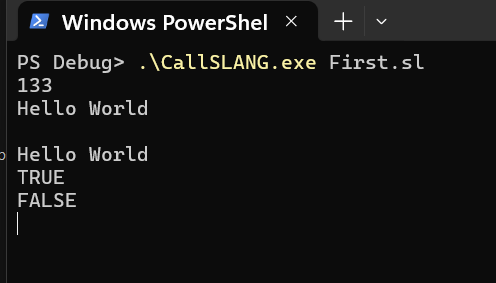
\includegraphics[width=0.5\textwidth]{first.png}

\chapter{Compilation to a .NET Executable}
Till now , the Slang Compiler was interpreting the statements and expressions. In this step we will try to compile the source into .net IL ( .net intermediate Language ). 

In this step, we are not going to make any change into the SLANG grammar. With Future ( support for Logical Expression, Relational Expression, Control structures and Procedures ) in mind, we will refactor the code. 

\section{Stack Based Machine Model}
.NET IL uses a Stack based machine model. Your Intel machines are register based. Stack based machine was touted as the future of machines in the early 1980s. What this basically means, the .NET CLR has got a evaluation stack for processing expressions and functions.... Read more about Reflection.Emit , CLR and IL to understand this.
To give a quick feel of what is involed, let us think about the expression 2*(3+4) 
This expression can be decomposed into
\lstset{style=csharp}
\begin{lstlisting}
	Acc = ADD 3 and 4 ( Acc stands for accumulator )
	Acc = Acc MUL 2 ;
\end{lstlisting}

if we are using a stack as an accumulator ( which .net does ) this can be written as
\lstset{style=csharp}
\begin{lstlisting}
	PUSH 3 // now stack contains [ 3 ]
	PUSH 4 // now stack constains [ 3, 4 ]
	ADD // pop 4 , pop 3 , add , push result
	// Now stack contains [ 7 ]
	PUSH 2 // Now stack conains [ 7, 2 ]
	MUL // pop 2 , pop 7 , multiply , push the result
	// now stack contains the result [ 14 ]
\end{lstlisting}
when the same stuff was compiled into .net ...this is what we got .....
\lstset{style=csharp}
\begin{lstlisting}
	// ---------------- IL output of 2*(3+4)
	IL_0000: ldc.r8 2. // push 2 [ 2 ]
	IL_0009: ldc.r8 3. // push 3 [ 2, 3 ]
	IL_0012: ldc.r8 4. // push 4 [ 2, 3, 4]
	IL_001b: add // pop 4 , pop 3 , add , push result [ 2, 7 ]
	IL_001c: mul // pop 7 , pop 2 , mul , push result [ 14 ]
\end{lstlisting}
The above output was generated using ILDASM.exe utility. That will help to disassemble .net executables.
\section{Execuatable}
In this chapter we compile all of the slang program into one main module.\\
To generate .NET executable , in the System.Reflection namespace there are some classes which we
need to be familiar.
\begin{verbatim}
AssemblyBuilder
ModuleBuilder
TypeBuilder
MethodBuilder
\end{verbatim}

From the name we can infer that these classes are based on GOF Builder pattern. The .NET StringBuilder class is another
notable class which is based on Builder pattern. Consult Wikipedia or a decent book on design patterns to learn more about
Builder Pattern. Later , we will be using Builder Pattern to Build (!) Procedure and Module from Program text.

An Assembly ( .NET exe or .net DLL ) is composed of Collection of Modules. In most cases , we will have one module per
assembly. Module will have collection of Types ( classes and structs ). Each Type will have collection of method. The
hierarchical relationonship between these entities are given below.

\begin{verbatim}
Hierarchy is as follows..
	Assembly
		Module
			Type
				Method
\end{verbatim}

For each entity there is a corresponding builder available. Please include System.Reflection and System.Reflection.Emit to
get access to these classes. How this has been used is given below.

\lstset{style=csharp}
\begin{lstlisting}
// Get The App Domain
AppDomain _app_domain = Thread.GetDomain();
AssemblyName _asm_name = new AssemblyName();
_asm_name.Name = "MyAssembly";

// Save the Exe Name
_name = name;

// Create an instance of Assembly Builder
_asm_builder = AppDomain.CurrentDomain.DefineDynamicAssembly(
_asm_name,
AssemblyBuilderAccess.RunAndSave);

// Create a module builder , from AssemblyBuilder
_module_builder = _asm_builder.DefineDynamicModule("DynamicModule1", _name, false);

// Create a class by the name MainClass..
// We compile the statements into a static method
// of the type MainClass .. the entry point will
// be called Main
_type_builder = _module_builder.DefineType("MainClass");
\end{lstlisting}
Now one can use Typebuilder instance to add methods to the type.
All the Executable creation logic has been included in a class by the name ExeGenerator.....
\lstset{style=csharp}
\begin{lstlisting}
// ExeGenerator - Takes care of the creation of
// .NET executable...
public class ExeGenerator
{
	//Hierarchy is as follows..
	// Assembly
	// 		Module
	// 			Type
	// 				Method
	// Refer to Reflection.Emit documentation for
	// more details on creation of .NET executable
	AssemblyBuilder _asm_builder = null;
	ModuleBuilder _module_builder = null;
	TypeBuilder _type_builder = null;

	// Name of the Executable
	string _name = "";
	// Program to be Compiled...
	TModule _p = null;
	public ExeGenerator(TModule p, string exeName)
	{
		// The Program to be compiled...
		_p = p;
		
		// Get The App Domain
		AppDomain _app_domain = Thread.GetDomain();
		AssemblyName _asm_name = new AssemblyName();
		
		// One can give a strong name , if we want
		_asm_name.Name = "MyAssembly";
		
		// Save the Exe Name
		_name = exeName;

		// Create an instance of Assembly Builder
		_asm_builder = 
			AppDomain.CurrentDomain.DefineDynamicAssembly(
				_asm_name,
				AssemblyBuilderAccess.RunAndSave);
		
		// Create a module builder , from AssemblyBuilder
		_module_builder = 
		_asm_builder.DefineDynamicModule("DynamicModule1", 
			_name, false);

		// Create a class by the name MainClass..
		// We compile the statements into a static method
		// of the type MainClass .. the entry point will
		// be called Main
		// ExeGenerator will be called from TModule.Compile method
		// We will add methods to the type MainClass as static method
		_type_builder = _module_builder.DefineType("MainClass");
	}
	
	// return the type builder....
	public TypeBuilder type_bulder
	{
		get { return _type_builder;}
	}
	
	public void Save()
	{
		// Note :- Call this (Save ) method only after
		// Compilation of All statements....
		_type_builder.CreateType();
		
		// Retrieve the Entry Point from TModule....
		MethodBuilder mb = _p._get_entry_point("MAIN");
		if (mb != null)
		{
			// Here we will set the Assembly 
			// as a Console Application...
			// We will also set the Entry Point....
			_asm_builder.SetEntryPoint(mb, 
				PEFileKinds.ConsoleApplication);
		}
		
		// Write the Resulting Executable...
		_asm_builder.Save(_name);
	}
}
\end{lstlisting}
\subsection{TModule.createExecutable}
The Above class will be called from TModule.CreateExecutable ( more about TModule later )
\lstset{style=csharp}
\begin{lstlisting}
public bool CreateExecutable(string name)
{
	// Create an instance of Exe Generator
	// ExeGenerator takes a TModule and
	// exe name as the Parameter...
	_exe = new ExeGenerator(this,name);
	// Compile The module...
	Compile(null);
	// Save the Executable...
	_exe.Save();
	return true;
}
\end{lstlisting}
\section{Generation Context}
To encapsulate the activities to be undertaken to Compile a Procedure to a static method, we have created a new class by the name, DNET\_EXECUTABLE\_GENERATION\_CONTEXT. For Compiling each Subroutine, an instance of this class will be created. This class contains\\
a ) ArrayList to store local variables...
\lstset{style=csharp}
\begin{lstlisting}
private ArrayList variables = new ArrayList();
\end{lstlisting}

b) Reference to an ILGenerator Object.
\lstset{style=csharp}
\begin{lstlisting}
private ILGenerator ILout;
\end{lstlisting}

c)SymbolTable for doing type analysis
\lstset{style=csharp}
\begin{lstlisting}
SymbolTable m_tab = new SymbolTable();
\end{lstlisting}
At this point of time , we are not supplying Procedure name to this class. We do not support user defined subroutines in this
step. This class only generates a method by the name MAIN.
By inspecting the Ctor of DNET\_EXECTUABLE\_GENERATION\_CONTEXT , we can get a fair idea of the usage of this
class...

\lstset{style=csharp}
\begin{lstlisting}
public DNET_EXECUTABLE_GENERATION_CONTEXT
(TModule program ,
Procedure proc,
TypeBuilder bld)
{
	// All the code in the Source module 
	// is compiled into this procedure
	_proc = proc;
	
	// TModule Object
	_program = program;

	// Handle to the type (MainClass )
	_bld = bld;
	
	// The method does not take any procedure
	System.Type[] s = null;
	
	// Return type is void
	System.Type ret_type = null;
	
	// public static void Main()
	_methinfo = _bld.DefineMethod("Main",
		MethodAttributes.Public | 
		MethodAttributes.Static,
		ret_type, s);
	// We have created the Method Prologue
	// Get the handle to the code generator
	ILout = _methinfo.GetILGenerator();
}
\end{lstlisting}
Creataion of Local Variables is not a difficult task. The ILGenerator class has got a method called DeclareLocal for that.
The following code snippet will explain the logic involved..

\lstset{style=csharp}
\begin{lstlisting}
public int DeclareLocal(System.Type type)
{
	// It is possible to create Local ( auto )
	// Variables by Calling DeclareLocl method
	// of ILGenerator... this returns an integer
	// We store this integer value in the variables
	// collection...
	LocalBuilder lb = ILout.DeclareLocal(type);

	// Now add the integer value associated with the
	// variable to variables collection...
	return variables.Add(lb);
}
\end{lstlisting}

The full code of DNET\_EXECUTABLE\_GENERATION\_CONTEXT class is given below.
\lstset{style=csharp}
\begin{lstlisting}
//DNET_EXECUTABLE_GENERATION_CONTEXT 
//is for generating
//CLR executable

public class DNET_EXECUTABLE_GENERATION_CONTEXT
{
	// ILGenerator Object
	private ILGenerator ILout;
	
	// Auto (Local) Variable support
	// Stores the index return by DefineLocal
	// method of MethodBuilder
	private ArrayList variables 
		= new ArrayList();

	// Symbol Table for storing Types and
	// doing the type analysis
	SymbolTable m_tab 
		= new SymbolTable();
	
	// CLR Reflection.Emit.MethodBuilder
	MethodBuilder _methinfo = null;
	
	// CLR Type Builder ( useful for creating
	// classes in the run time
	TypeBuilder _bld=null;

	// Procedure to compiled
	Procedure _proc = null;
	// Program to be compiled...
	TModule _program;
	public DNET_EXECUTABLE_GENERATION_CONTEXT
		(TModule program ,
		Procedure proc,
		TypeBuilder bld)
	{
		// All the code in the Source module 
		// is compiled
		// into this procedure
		_proc = proc;
		
		// TModule Object
		_program = program;
		
		// Handle to the type (MainClass )
		_bld = bld;
		
		// The method does not take any procedure
		System.Type[] s = null;
		
		// Return type is void
		System.Type ret_type = null;

		// public static void Main()
		_methinfo = _bld.DefineMethod("Main",
			MethodAttributes.Public | 
			MethodAttributes.Static,
			ret_type, s);
		
		// We have created the Method Prologue
		// Get the handle to the code generator
		ILout = _methinfo.GetILGenerator();
	}
	
	public string MethodName
	{
		get{return _proc.Name ;}
	}
 
	public MethodBuilder MethodHandle
	{
		get{return _methinfo;}
	}
	
	public TypeBuilder TYPEBUILDER
	{
		get{return _bld;}
	}

	public SymbolTable TABLE
	{
		get{return m_tab;}
	}
	
	public ILGenerator CodeOutput
	{	
		get{return ILout;}
	}
	
	public int DeclareLocal(System.Type type)
	{
		// It is possible to create Local ( auto )
		// Variables by Calling DeclareLocl method
		// of ILGenerator... this returns an integer
		// We store this integer value in the variables
		// collection...
		LocalBuilder lb = ILout.DeclareLocal(type);
		
		// Now add the integer value associated with the
		// variable to variables collection...
		return variables.Add(lb);
	}
	
	public LocalBuilder GetLocal(int s)
	{
		return variables[s] as LocalBuilder;
	}
}
\end{lstlisting}
\clearpage
\section{Compiling Expressions}
\subsection{Exp}
To support compilation into .NET IL for expressions, we have an addional method appropriately named Compile to the Exp base class.

\lstset{style=csharp}
\begin{lstlisting}
// In this Step , we add two more methods to the Exp class
// TypeCheck => To do Type analysis
// get_type => Type of this node
public abstract class Exp
{
	public abstract SYMBOL_INFO Evaluate(
	RUNTIME_CONTEXT cont);
	
	public abstract TYPE_INFO TypeCheck(
	COMPILATION_CONTEXT cont);
	
	public abstract TYPE_INFO get_type();
	
	// Added in the STEP 5 for .NET IL 
	// code generation
	public abstract bool 
	Compile(DNET_EXECUTABLE_GENERATION_CONTEXT cont);
}
\end{lstlisting}
This additional method takes a \\
DNET\_EXECUTABLE\_GENERATION\_CONTEXT as the parameter.
\subsection{NumericConstant}
To generate Code for Loading a NumericConstant ....this what we one has to do ....
\lstset{style=csharp}
\begin{lstlisting}
public override bool 
Compile(DNET_EXECUTABLE_GENERATION_CONTEXT cont)
{
	// Emit LDC_R8 => Load Constant Real 8
	// IEEE 754 floating Point
	// cont.CodeOutput will return ILGenerator of the
	// current method...
	cont.CodeOutput.Emit(OpCodes.Ldc_R8, 
		info.dbl_val);
	return true;
}
\end{lstlisting}
\subsection{BooleanConstant}
The code emitted for a BooleanConstant:

\lstset{style=csharp}
\begin{lstlisting}
public override bool 
Compile(DNET_EXECUTABLE_GENERATION_CONTEXT cont)
{
	// Retrieve the IL Code generator and Emit
	// LDC_I4 => Load Constant Integer 4
	// We are planning to use a 32 bit long for Boolean
	// True or False
	cont.CodeOutput.Emit(OpCodes.Ldc_I4, 
		(info.bol_val) ? 1 : 0);
	return true;
}
\end{lstlisting}

\subsection{StringLiteral}
The code emitted for a StringLiteral:

\lstset{style=csharp}
\begin{lstlisting}
public override bool 
Compile(DNET_EXECUTABLE_GENERATION_CONTEXT cont)
{
	// For string emit
	// LDSTR => Load String
	cont.CodeOutput.Emit(OpCodes.Ldstr , 
		info.str_val);
	return true;
}
\end{lstlisting}
\subsection{Variable}
The Code emitted for loading a variable reference on to the stack:
\lstset{style=csharp}
\begin{lstlisting}
public override bool 
Compile(DNET_EXECUTABLE_GENERATION_CONTEXT cont)
{
	// Retrieve the Symbol information from the
	// Symbol Table. Symbol name is the key here..
	SYMBOL_INFO info 
		= cont.TABLE.Get(m_name);

	// Give the Position to retrieve 
	// the Local Variable Builder.
	LocalBuilder lb 
		= cont.GetLocal(info.loc_position);

	// LDLOC => Load Local... we need to give
	// a Local Builder as parameter
	cont.CodeOutput.Emit(
		OpCodes.Ldloc, lb);
	return true;
}
\end{lstlisting}

\subsection{BinaryPlus}
The Code emitted for BinaryPlus (+) needs to query the operand to generate the appropriate code. If the Left and the right expression is numeric... it needs to Generate Add opcode. There is no appropriate operator for String Concatenation. One needs to use String.Concat method to do that....

\lstset{style=csharp}
\begin{lstlisting}
public override bool 
Compile(DNET_EXECUTABLE_GENERATION_CONTEXT cont)
{
	// Compile the Left Expression
	exp1.Compile(cont);
	
	// Compile the Right Expression
	exp2.Compile(cont);

	// Emit Add instruction

	if (_type == TYPE_INFO.TYPE_NUMERIC)
	{
		cont.CodeOutput.Emit(OpCodes.Add);
	}
	else
	{
		// This is a string type..we need to call
		// Concat method..
		Type[] str2 = {
			typeof(string),
			typeof(string)
		};
		cont.CodeOutput.Emit(OpCodes.Call,
			typeof(String).GetMethod("Concat", str2));
	}
	return true;
}
\end{lstlisting}
For this routine to work correctly , one needs to call TypeCheck every time to update the type information on all nodes.. This polymorphic behavior forced us to call TypeCheck every time we finished parsing an expression.

\lstset{style=csharp}
\begin{lstlisting}
private Stmt 
ParsePrintStatement(ProcedureBuilder ctx)
{
	GetNext();
	Exp a = Expr(ctx);
	
	// Do the type analysis ...
	a.TypeCheck(ctx.Context);
	if (Current_Token != TOKEN.TOK_SEMI)
	{
		throw new Exception("; is expected");
	}
	return new PrintStatement(a);
}
\end{lstlisting}

\subsection{BinaryMinus}
The code generation of Subtract Operation is as follows.

\lstset{style=csharp}
\begin{lstlisting}
public override bool 
Compile(DNET_EXECUTABLE_GENERATION_CONTEXT cont)
{
	exp1.Compile(cont);
	exp2.Compile(cont);
	cont.CodeOutput.Emit(OpCodes.Sub);
	return true;
}
\end{lstlisting}

\subsection{UnaryMinus}
The code emitted for UnaryMinus is as given below.

\lstset{style=csharp}
\begin{lstlisting}
public override bool 
Compile(DNET_EXECUTABLE_GENERATION_CONTEXT cont)
{
	// Compile the expression
	exp1.Compile(cont);
	
	// Negate the value on the top of the
	// stack
	cont.CodeOutput.Emit(OpCodes.Neg);
	return true;
}
\end{lstlisting}
\section{Compiling Statements}
\subsection{Stmt}
To support the Compilation of statement into IL an additional method has been added to the Stmt base class.
\lstset{style=csharp}
\begin{lstlisting}
public abstract class Stmt
{
	public abstract SYMBOL_INFO 
	Execute(RUNTIME_CONTEXT cont);

	// Added in the Step 5 for .net IL compilation
	public abstract bool 
	Compile(DNET_EXECUTABLE_GENERATION_CONTEXT cont);
}
\end{lstlisting}
\subsection{PrintStatement}
The Code emitted for PrintStatement is given below.
\lstset{style=csharp}
\begin{lstlisting}
public override bool 
Compile(DNET_EXECUTABLE_GENERATION_CONTEXT cont)
{
	// Compile the Expression
	// The Output will be on the top of stack
	exp1.Compile(cont);
	
	// Generate Code to Call Console.Write
	System.Type typ = Type.GetType("System.Console");
	Type[] Parameters = new Type[1];
	TYPE_INFO tdata = exp1.get_type();
	if (tdata == TYPE_INFO.TYPE_STRING)
		Parameters[0] = typeof(string);
	else if (tdata == TYPE_INFO.TYPE_NUMERIC)
		Parameters[0] = typeof(double);
	else
		Parameters[0] = typeof(bool);
	cont.CodeOutput.Emit(OpCodes.Call, 
		typ.GetMethod("Write", Parameters));
	return true;
}
\end{lstlisting}
\subsection{VariableDeclStatement}
The Code emitted for VariableDeclStatement is as follows.

\lstset{style=csharp}
\begin{lstlisting}
public override bool 
Compile(DNET_EXECUTABLE_GENERATION_CONTEXT cont)
{

	// Retrieve the type from the SYMBOL_INFO
	System.Type type 
		= (m_inf.Type == TYPE_INFO.TYPE_BOOL) ?
		typeof(bool) : 
		(m_inf.Type == TYPE_INFO.TYPE_NUMERIC) ?
			typeof(double) : 
		typeof(string);

	// Get the offset of the variable
	int s = cont.DeclareLocal(type);

	// Store the offset in the SYMBOL_INFO
	m_inf.loc_position = s;
	
	// Add the variable into Symbol Table..
	cont.TABLE.Add(m_inf);
	return true;
}
\end{lstlisting}
\subsection{AssignmentStatement}
The code for the Assignment statement is as given below.
\lstset{style=csharp}
\begin{lstlisting}
public override bool 
Compile(DNET_EXECUTABLE_GENERATION_CONTEXT cont)
{
	if (!exp1.Compile(cont))
	{
		throw new 
		Exception(
		"Compilation in error string");
	}
	SYMBOL_INFO info 
		= cont.TABLE.Get(variable.Name);
	LocalBuilder lb 
		= cont.GetLocal(info.loc_position);
	cont.CodeOutput.Emit(OpCodes.Stloc, lb);
	return true;
}
\end{lstlisting}

\section{PROC}
To support additional language constructs , we had two additional base classes in this project. The class Procedure is to model a FUNCTION. At this point we compile all the statement into a Function. In future, we will support User defined Function.
\lstset{style=csharp}
\begin{lstlisting}
// Abstract base class for Procedure
// All the statements in a Program ( Compilation unit )
// will be compiled into a PROC
public abstract class PROC
{
	public abstract SYMBOL_INFO 
	Execute(RUNTIME_CONTEXT cont);
	
	public abstract bool 
	Compile(DNET_EXECUTABLE_GENERATION_CONTEXT cont);
}
\end{lstlisting}
\subsection{Procedure}
The Concrete class Procedure implements in this interface.
\lstset{style=csharp}
\begin{lstlisting}
public class Procedure : PROC
{
	// Procedure name ..which defaults to Main
	// in the type MainClass
	public string 
		m_name;
	
	// Formal parameters...	
	public ArrayList 
		m_formals = null;
		
	// List of statements which comprises 
	// the Procedure
	public ArrayList 
		m_statements = null;

	// Local variables
	public SymbolTable 
		m_locals = null;

	// return_value.... a hard coded zero 
	// at this point of time..
	public SYMBOL_INFO 
		return_value = null;
	

	// TYPE_INFO => TYPE_NUMERIC
	public TYPE_INFO 
		_type = TYPE_INFO.TYPE_ILLEGAL;
	
	// Rest of the Code
	
}
\end{lstlisting}
Let us look at the Compile method of the Procedure class. Procedure is nothing but a collection of staements.

\lstset{style=csharp}
\begin{lstlisting}
public override bool 
Compile(DNET_EXECUTABLE_GENERATION_CONTEXT cont)
{
	foreach (Stmt e1 in m_statements)
	{
		e1.Compile(cont);
	}
	cont.CodeOutput.Emit(OpCodes.Ret);
	return true;
}
\end{lstlisting}

The Execute method of the Procedure is very similar to Compile method. Instead of Calling Compile method , Execute will delegate the call to Execute mathod of statement.

\lstset{style=csharp}
\begin{lstlisting}
public override SYMBOL_INFO 
Execute(RUNTIME_CONTEXT cont)
{
	foreach (Stmt stmt in m_statements)
		stmt.Execute(cont);
	return null;
}
\end{lstlisting}

\section{Module}
Another interface defined is to support the concept of a module. Module ( at this point of time ) is just collection of
statements. The collection of statements will be compiled into a Procedure. And the Procedure will embedded in a module.
\footnote{When we support user defined Functions , the meaning of module will be changed a bit. Then the Module will become
collection of Functions.} All the Functions will be compiled as static methods of a single type. One can easily extend the
compiler to support classes.

\lstset{style=csharp}
\begin{lstlisting}
// A bunch of statement is called a Compilation
// unit at this point of time... STEP 5
// In future , a Collection of Procedures will be
// called a Compilation unit
// Added in the STEP 5
public abstract class 
CompilationUnit
{
	public abstract SYMBOL_INFO Execute(
	RUNTIME_CONTEXT cont);

	public abstract bool 
	Compile(DNET_EXECUTABLE_GENERATION_CONTEXT cont);
}
\end{lstlisting}
Since there is a preexisting type called Module available in the .net class hierarchy, we will use the name TModule instead.

\lstset{style=csharp}
\begin{lstlisting}
// A CodeModule is a Compilation Unit ..
// At this point of time ..it is just a bunch
// of statements...
public class TModule : CompilationUnit
{
	// A Program is a collection of Procedures...
	// Now , we support only global function...
	private ArrayList m_procs=null;
	// List of Compiled Procedures....
	// At this point of time..only one procedure
	// will be there....
	private ArrayList compiled_procs = null;

	// class to generate IL executable...
	private ExeGenerator _exe = null;

	// Ctor for the Program ...
	public TModule(ArrayList procs)
	{
		m_procs = procs;
	}
	
	public bool 
	CreateExecutable(string name)
	{
		// Create an instance of Exe Generator
		// ExeGenerator takes a TModule and
		// exe name as the Parameter...
		_exe = new ExeGenerator(this,name);
		
		// Compile The module...
		Compile(null);
		
		// Save the Executable...
		_exe.Save();
		return true;
	}
	public override bool 
	Compile(DNET_EXECUTABLE_GENERATION_CONTEXT cont)
	{
	
		compiled_procs = new ArrayList();
	
		foreach (Procedure p in m_procs)
		{
			DNET_EXECUTABLE_GENERATION_CONTEXT con
			= new
			DNET_EXECUTABLE_GENERATION_CONTEXT(
				this,p, _exe.type_bulder);
			compiled_procs.Add(con);
			p.Compile(con);
		}
		return true;
	}
	
	public override SYMBOL_INFO Execute(
		RUNTIME_CONTEXT cont)
	{
		Procedure p = Find("Main");
		if (p != null)
		{
			return p.Execute(cont);
		}
		return null;
	}
	
	public MethodBuilder _get_entry_point(
		string _funcname)
	{
		foreach (
		DNET_EXECUTABLE_GENERATION_CONTEXT u 
		in compiled_procs)
		{
			if (u.MethodName
				.Equals(_funcname))
			{
				return u.MethodHandle;
			}
		}
		return null;
	}
	
	public Procedure Find(string str)
	{
		foreach (Procedure p in m_procs)
		{
			string pname = p.Name;
			if (pname.ToUpper()
			.CompareTo(str.ToUpper()) == 0)
			return p;
		}
		return null;
	}
}
\end{lstlisting}

\section{Builders}
To create TModule and Procedure Object , we need to Parse the statemeents. We can create the Objects only when we have
finished the Parsing. We need to accumulate the requisite Objects before we create Procedure. Builder Pattern is a nice way
to organize the code to do these kind of stuff.
\lstset{style=csharp}
\begin{lstlisting}
// Base class for all the Builder
// AbstractBuilder
// TModuleBuilder
// ProcedureBuilder
public class AbstractBuilder
{
}
\end{lstlisting}
\subsection{TModuleBuilder}
The Source code of the Module Builder is given below.
\lstset{style=csharp}
\begin{lstlisting}
// A Builder for Creating a Module
class TModuleBuilder : AbstractBuilder
{
	// Array of Procs
	private ArrayList procs;

	// Array of Function Prototypes
	// not much use as of now...
	private ArrayList protos=null;

	// Ctor does not do much
	public TModuleBuilder()
	{
		procs = new ArrayList();
		protos = null;
	}
	
	// Add Procedure
	public bool Add(Procedure p)
	{
		procs.Add(p);
		return true;
	}

	// Create Program
	public TModule GetProgram()
	{
		return new TModule(procs);
	}
	
	public Procedure GetProc(string name)
	{
		foreach (Procedure p in procs)
		{
			if (p.Name.Equals(name))
			{
				return p;
			}
		}
		return null;
	}
}
\end{lstlisting}
\subsection{ProcedureBuilder}
The source code of the ProcedureBuilder is given below...
\lstset{style=csharp}
\begin{lstlisting}
	public class ProcedureBuilder
		: AbstractBuilder
	{

		// Procedure name ..now it is hard coded
		// to MAIN
		private string proc_name = "";
		
		// Compilation context for type analysis
		COMPILATION_CONTEXT ctx = null;

		// Procedure does not take any argument..
		ArrayList m_formals = null;
		
		// Array of Statements
		ArrayList m_stmts = new ArrayList();

		// Return Type of the procedure
		TYPE_INFO inf = TYPE_INFO.TYPE_ILLEGAL;
		public ProcedureBuilder(
			string name, COMPILATION_CONTEXT _ctx)
		{
			ctx = _ctx;
			proc_name = name;
		}

		public bool AddLocal(
			SYMBOL_INFO info)
		{
			ctx.TABLE.Add(info);
			return true;
		}
		
		public TYPE_INFO TypeCheck(
			Exp e)
		{
			return e.TypeCheck(ctx);
		}

		public void AddStatement(
			Stmt st)
		{
			m_stmts.Add(st);
		}
		
		public SYMBOL_INFO 
		GetSymbol(string strname)
		{
			return ctx
				.TABLE.Get(strname);
		}

		// Check the function Prototype
		public bool 
		CheckProto(string name)
		{
			return true;
		}
		
		public TYPE_INFO TYPE
		{
			get{return inf;}
			set{inf = value;}
		}
		
		public SymbolTable TABLE
		{
			get{return ctx.TABLE;}
		}
		
		public COMPILATION_CONTEXT 
		Context
		{
			get{return ctx;}
		}
		
		public string Name
		{
			get{return proc_name;}
			set{proc_name = value;}
		}
		
		public Procedure 
		GetProcedure()
		{
			Procedure ret 
			= new Procedure(proc_name,
				m_stmts, ctx.TABLE, inf);
			return ret;
		}
}
\end{lstlisting}
\section{Parse Process}
The Parse Process in the RDParser modules starts from the DoParse Method.

\lstset{style=csharp}
\begin{lstlisting}
public TModule DoParse()
{
	ProcedureBuilder p = 
	new ProcedureBuilder(
	"MAIN", 
	new COMPILATION_CONTEXT());
	
	ArrayList stmts = Parse(p);
	foreach (Stmt s in stmts)
	{
		p.AddStatement(s);
	}
	Procedure pc 
		= p.GetProcedure();
	prog.Add(pc);
	return prog.GetProgram();
}
\end{lstlisting}
\subsection{Using ParserBuilder}
In this version all the methods in the Parser takes a ProcedureBuilder object as parameter...
\lstset{style=csharp}
\begin{lstlisting}
private ArrayList 
StatementList(ProcedureBuilder ctx)
{
	ArrayList arr = new ArrayList();
	while (Current_Token 
		!= TOKEN.TOK_NULL)
	{
		Stmt temp = Statement(ctx);
		if (temp != null)
		{
			arr.Add(temp);
		}
	}
	return arr;
}
\end{lstlisting}
In the previous step , these routines were taking a COMPILATION\_CONTEXT as paramter. In this step , this object is encapsulated in ProcedureBuilder object.

\section{Projects}
Now onwards, we will have three projects in the solution.\\
SLANG\_DOT\_NET $\rightarrow$ Compilation Engine\\
SLANGCOMPILE $\rightarrow$ Calls the Compilation Engine to generate .NET executable\\
SLANGINTERPRET $\rightarrow$ Calls the Compilation Engine to interpret the statements\\
\subsection{SLANGCOMPILE}
Let us take a look at the source code of SLANGCOMPILE.
\lstset{style=csharp}
\begin{lstlisting}
using System;
using System.Collections;
using System.Linq;
using System.Text;
using System.IO;
using SLANG_DOT_NET;
namespace SLANGCOMPILE {
class Caller
{
	// Driver routine to call the program script
	static void TestFileScript(string filename)
	{
		if (filename == null)
		return;
		
		//Read the contents from the file
		StreamReader sr = new StreamReader(filename);
		string programs2 = sr.ReadToEnd();
		sr.Close();
		sr.Dispose();
		
		//Creates the Parser Object
		// With Program text as argument
		RDParser pars = null;
		pars = new RDParser(programs2);
		TModule p = null;
		p = pars.DoParse();
		
		// Now that Parse is Successul...
		// Create an Executable...!
		if (p.CreateExecutable("First.exe"))
		{
			Console.WriteLine(
				"Creation of Executable is successul");
			return;
		}
	}
	
	static void Main(string[] args)
	{
		if (args == null ||
			args.Length != 1)
		{
			Console.WriteLine(
				"SLANGCOMPILE <scriptname>\n");
			return;
		}
		
		TestFileScript(args[0]);
		
		//Wait for the Key Press
		Console.Read();
	}
}
}
\end{lstlisting}
\subsection{SLANGINTERPRET}
The source code of the SLANGINTERPRET is as given below.
\lstset{style=csharp}
\begin{lstlisting}
using System;
using System.Collections.Generic;
using System.Linq;
using System.Text;
using System.Collections;
using System.IO;
using SLANG_DOT_NET;
namespace CallSLANG{
class Caller
{

	// Driver routine to call the program script
	static void TestFileScript(string filename)
	{
		if (filename == null)
		return;
		
		//Read the contents from the file
		StreamReader sr 
			= new StreamReader(filename);
		string programs2 
			= sr.ReadToEnd();
		
		//Creates the Parser Object
		// With Program text as argument
		RDParser pars = null;
		pars = new RDParser(programs2);
		TModule p = null;
		p = pars.DoParse();
		
		// Now that Parse is Successul...
		// Do a recursive interpretation...!
		RUNTIME_CONTEXT f 
			= new RUNTIME_CONTEXT(p);
		SYMBOL_INFO fp 
			= p.Execute(f);
	}
	
	static void Main(string[] args)
	{
		if (args == null ||
			args.Length != 1)
		{
			Console.WriteLine(
				"SLANGINTERPRET <scriptname>\n");
			return;
		}
		TestFileScript(args[0]);
		
		//Wait for the Key Press
		Console.Read();
	}
}
}
\end{lstlisting}
\section{Outputs}
Let us check how our compiler has generated code for some scripts.
\subsection{Example 1}
\lstset{style=csharp}
\begin{lstlisting}
PRINTLINE 2*(3+4);
\end{lstlisting}

Using the ILDASM utility , here is what we get from our compiler...

\lstset{style=csharp}
\begin{lstlisting}
.method public static void Main() cil managed
{
	.entrypoint
	// Code size 35 (0x23)
	.maxstack 3
	IL_0000: ldc.r8 2.
	IL_0009: ldc.r8 3.
	IL_0012: ldc.r8 4.
	IL_001b: add
	IL_001c: mul
	IL_001d: call void [mscorlib]System.Console::WriteLine(float64)
	IL_0022: ret
}
// end of method MainClass::Main
\end{lstlisting}
\subsection{Example 2}
String concatenation.
\lstset{style=csharp}
\begin{lstlisting}
PRINT "Hello World" + " SL ";
\end{lstlisting}

The output generated by our compiler was as follows.

\lstset{style=csharp}
\begin{lstlisting}
.method public static void Main() cil managed
{
	.entrypoint
	// Code size 21 (0x15)
	.maxstack 2
	IL_0000: ldstr "Hello World"
	IL_0005: ldstr " SL "
	IL_000a: call string [mscorlib]System.String::Concat(string, string)
	IL_000f: call void [mscorlib]System.Console::Write(string)
	IL_0014: ret
} // end of method MainClass::Main
\end{lstlisting}

\subsection{Example 3}
Unary expression.
\lstset{style=csharp}
\begin{lstlisting}
Numeric a;
String b;
a = ---1;
PrintLine a*4 + 10;
\end{lstlisting}

The code generated by the compiler is as follows.

\lstset{style=csharp}
\begin{lstlisting}
.method public static void Main() cil managed
{
	.entrypoint
	// Code size 40 (0x28)
	.maxstack 2
	.locals init (float64 V_0,
	string V_1)
	IL_0000: ldc.r8 1.
	IL_0009: neg
	IL_000a: neg
	IL_000b: neg
	IL_000c: stloc.0
	IL_000d: ldloc.0
	IL_000e: ldc.r8 4.
	IL_0017: mul
	IL_0018: ldc.r8 10.
	IL_0021: add
	IL_0022: call void [mscorlib]System.Console::WriteLine(float64)
	IL_0027: ret
} // end of method MainClass::Main
\end{lstlisting}

\subsection{Example 4}
The following script test allmost all the features of the compiler ( implemented at this point of time )
\lstset{style=csharp}
\begin{lstlisting}
NUMERIC a; // Declare a Numeric variable
a = 2*3+5* 30 + -(4*5+3); // Assign
PRINTLINE a; // Dump a
/
/String concatenation
PRINT "Hello " + "World";

//Write a new line
PRINTLINE "";

//string data type
STRING c;
c = "Hello "; // assignment to string

//assignment and concatenation
C = C + "World";
PRINTLINE c;

//boolean variable
BOOLEAN d;
d= TRUE;
PRINTLINE d;
d= FALSE;
PRINTLINE d;
\end{lstlisting}

The output is:

\lstset{style=csharp}
\begin{lstlisting}
.method public static void Main() cil managed
{
	.entrypoint
	// Code size 156 (0x9c)
	.maxstack 4
	.locals init (float64 V_0,
		string V_1,
		bool V_2)
	IL_0000: ldc.r8 2.
	IL_0009: ldc.r8 3.
	IL_0012: mul
	IL_0013: ldc.r8 5.
	IL_001c: ldc.r8 30.
	IL_0025: mul
	IL_0026: ldc.r8 4.
	IL_002f: ldc.r8 5.
	IL_0038: mul
	IL_0039: ldc.r8 3.
	IL_0042: add
	IL_0043: neg
	IL_0044: add
	IL_0045: add
	IL_0046: stloc.0
	IL_0047: ldloc.0
	IL_0048: call void [mscorlib]System.Console::WriteLine(float64)
	IL_004d: ldstr "Hello "
	IL_0052: ldstr "World"
	IL_0057: call string [mscorlib]System.String::Concat(string,string)
	IL_005c: call void [mscorlib]System.Console::Write(string)
	IL_0061: ldstr ""
	IL_0066: call void [mscorlib]System.Console::WriteLine(string)
	IL_006b: ldstr "Hello "
	IL_0070: stloc.1
	IL_0071: ldloc.1
	IL_0072: ldstr "World"
	IL_0077: call string [mscorlib]System.String::Concat(string,string)
	IL_007c: stloc.1
	IL_007d: ldloc.1
	IL_007e: call void [mscorlib]System.Console::WriteLine(string)
	IL_0083: ldc.i4 0x1
	IL_0088: stloc.2
	IL_0089: ldloc.2
	IL_008a: call void [mscorlib]System.Console::WriteLine(bool)
	IL_008f: ldc.i4 0x0
	IL_0094: stloc.2
	IL_0095: ldloc.2
	IL_0096: call void [mscorlib]System.Console::WriteLine(bool)
	IL_009b: ret
} // end of method MainClass::Main
\end{lstlisting}
\chapter{Control Structures}
In this step, we will support Control Structures like IF statement and While Statement. Before we begin, we need to extend the Exp hierarchy with Relational Expression and Logical Exp	ressions. 

\section{Tokens}
Let us extend the list of tokens with Additonal Tokens for Relational expressions, Logical Expressions and Control structures.
\lstset{style=csharp}
\begin{lstlisting}
// ----------- Added in Step 6
// for relational operator support
TOK_EQ, // '=='
TOK_NEQ, // '<>'
TOK_GT, // '>'
TOK_GTE, // '>='
TOK_LT, // '<'
TOK_LTE, // '<='
TOK_AND, // '&&'
TOK_OR, // '||'
TOK_NOT, // '!'
//------------ Added in Step 6 for
// Control structures support
TOK_IF, // IF
TOK_THEN, // Then
TOK_ELSE, // Else Statement
TOK_ENDIF, // Endif Statement
TOK_WHILE, // WHILE
TOK_WEND // Wend Statement
\end{lstlisting}

Additonal Keywords supported include:
\lstset{style=csharp}
\begin{lstlisting}
// -------------- Added in the step 6
// -------------- To support control structures
keyword[7] = new ValueTable(TOKEN.TOK_IF, "IF");
keyword[8] = new ValueTable(TOKEN.TOK_WHILE, "WHILE");
keyword[9] = new ValueTable(TOKEN.TOK_WEND, "WEND");
keyword[10] = new ValueTable(TOKEN.TOK_ELSE, "ELSE");
keyword[11] = new ValueTable(TOKEN.TOK_ENDIF, "ENDIF");
keyword[12] = new ValueTable(TOKEN.TOK_THEN, "THEN");
\end{lstlisting}

We need to create a new enum for Relational Operators.

\lstset{style=csharp}
\begin{lstlisting}
// Relational Operators
public enum RELATION_OPERATOR
{
	TOK_EQ, // '=='
	TOK_NEQ, // '<>'
	TOK_GT, // '>'
	TOK_GTE, // '>='
	TOK_LT, // '<'
	TOK_LTE, // '<='
}
\end{lstlisting}
\section{Supporting Relational Expressions}
Now we have got everything ready to write a class for Relational Expression.
\subsection{R.E. Class Vars}
\lstset{style=csharp}
\begin{lstlisting}
public class RelationExp : Exp
{
	// Which Operator
	RELATION_OPERATOR m_op;
	
	// Left and Right Expression
	private Exp ex1, ex2;
	
	// Type of this node
	TYPE_INFO _type;

	// Operand Types .. if operands are string
	// we need to generate call to String.Compare
	// method...
	TYPE_INFO _optype;
	
	//Rest of the code...
}
\end{lstlisting}
\subsection{Evaluate Routine}
Let us take a look at the Evaluate routine. The Evaluate routine will give good insight into the implementation of Relational Expression. The basic idea is to Evaluate the Left Expression ( Exp1 ) and Right Expression (Exp2 ). Once the evaluation is over , one can query the Operand Type ( The Operands need to be of same type ) and perform the appropriae action.\\

For Boolean and String type, only \texttt{==} and \texttt{<>} are supported. The TypeChecking routine makes sure that only these operands are permited for Boolean and String Type.


\lstset{style=csharp}
\begin{lstlisting}
// The logic of this method is obvious...
// Evaluate the Left and Right Expression...
// Query the Type of the expressions and perform
// appropriate action
public override SYMBOL_INFO 
Evaluate(RUNTIME_CONTEXT cont)
{
	SYMBOL_INFO eval_left = ex1.Evaluate(cont);
	SYMBOL_INFO eval_right = ex2.Evaluate(cont);
	SYMBOL_INFO ret_val = new SYMBOL_INFO();
	if (eval_left.Type 
			== TYPE_INFO.TYPE_NUMERIC &&
		eval_right.Type 
			== TYPE_INFO.TYPE_NUMERIC)
	{
		ret_val.Type 
			= TYPE_INFO.TYPE_BOOL;
		ret_val.SymbolName = "";
		if (m_op == RELATION_OPERATOR.TOK_EQ) {
			ret_val.bol_val 
			= eval_left.dbl_val == eval_right.dbl_val;
		}
		else if (m_op == RELATION_OPERATOR.TOK_NEQ) {
			ret_val.bol_val 
			= eval_left.dbl_val != eval_right.dbl_val;
		}
		else if (m_op == RELATION_OPERATOR.TOK_GT) {
			ret_val.bol_val 
			= eval_left.dbl_val > eval_right.dbl_val;
		}
		else if (m_op == RELATION_OPERATOR.TOK_GTE) {
			ret_val.bol_val 
			= eval_left.dbl_val >= eval_right.dbl_val;
		}
		else if (m_op == RELATION_OPERATOR.TOK_LTE) {
			ret_val.bol_val 
			= eval_left.dbl_val <= eval_right.dbl_val;
		}
		else if (m_op == RELATION_OPERATOR.TOK_LT) {
			ret_val.bol_val 
				= eval_left.dbl_val < eval_right.dbl_val;
			return ret_val;
		}
	}
	else if (eval_left.Type == TYPE_INFO.TYPE_STRING &&
		eval_right.Type == TYPE_INFO.TYPE_STRING)
	{
		ret_val.Type = TYPE_INFO.TYPE_BOOL;
		ret_val.SymbolName = "";
		if (m_op == RELATION_OPERATOR.TOK_EQ)
		{
			ret_val.bol_val = ( String.Compare(
			eval_left.str_val,
			eval_right.str_val) == 0 ) ? true:false;
		}
		else if (m_op == RELATION_OPERATOR.TOK_NEQ)
		{
			ret_val.bol_val = String.Compare(
			eval_left.str_val,
			eval_right.str_val) != 0;
		}
		else
		{
			ret_val.bol_val = false;
		}
		return ret_val;
	}
	if (eval_left.Type == TYPE_INFO.TYPE_BOOL &&
		eval_right.Type == TYPE_INFO.TYPE_BOOL)
	{
		ret_val.Type = TYPE_INFO.TYPE_BOOL;
		ret_val.SymbolName = "";
		if (m_op == RELATION_OPERATOR.TOK_EQ) {
			ret_val.bol_val
			= eval_left.bol_val == eval_right.bol_val;
		}
		else if (m_op == RELATION_OPERATOR.TOK_NEQ) {
			ret_val.bol_val
			= eval_left.bol_val != eval_right.bol_val;
		}
		else {
			ret_val.bol_val = false;
		}
		return ret_val;
	}
	return null;
}
\end{lstlisting}
\subsection{Type Checking}
Let us take a look at TypeCheck routine of RelationalExp class.
\lstset{style=csharp}
\begin{lstlisting}
// Recursively check the type and bubble up the type
// information to the top...
public override TYPE_INFO 
TypeCheck(COMPILATION_CONTEXT cont)
{
	TYPE_INFO eval_left = ex1.TypeCheck(cont);
	TYPE_INFO eval_right = ex2.TypeCheck(cont);
	if (eval_left != eval_right)
	{
		throw 
		new Exception("Wrong Type in expression");
	}
	
	if (eval_left == TYPE_INFO.TYPE_STRING &&
		(!(m_op == RELATION_OPERATOR.TOK_EQ ||
		m_op == RELATION_OPERATOR.TOK_NEQ)))
	{
		throw new 
		Exception("Only == and != supported for string type ");
	}

	if (eval_left == TYPE_INFO.TYPE_BOOL &&
		(!(m_op == RELATION_OPERATOR.TOK_EQ ||
		m_op == RELATION_OPERATOR.TOK_NEQ)))
	{
		throw new 
		Exception("Only == and != supported for boolean type ");
	}
 
	// store the operand type as well
	_optype = eval_left;
	_type = TYPE_INFO.TYPE_BOOL;
	return _type;
}
\end{lstlisting}
\subsection{Compile String R.E.}
To Compile a RelationalExpression involving String Operands ( \texttt{==} and \texttt{<>} ), we need to generate calls to String.Compare method.
\lstset{style=csharp}
\begin{lstlisting}
private bool 
CompileStringRelOp(
	DNET_EXECUTABLE_GENERATION_CONTEXT cont)
{
	
	// Compile the Left Expression
	ex1.Compile(cont);

	// Compile the Right Expression
	ex2.Compile(cont);
	// This is a string type..we need to call
	// Compare method..
	Type[] str2 = {
		typeof(string),
		typeof(string)
	};
	cont.CodeOutput.Emit(OpCodes.Call,
		typeof(String).GetMethod("Compare", str2));
	if (m_op == RELATION_OPERATOR.TOK_EQ)
	{
		cont.CodeOutput.Emit(OpCodes.Ldc_I4, 0);
		cont.CodeOutput.Emit(OpCodes.Ceq);
	}
	else
	{
	
		// This logic is bit convoluted...
		// String.Compare will give 0 , 1 or -1
		// First we will check whether the stack value
		// is zero..
		// This will put 1 on stack ..if value was zero
		// after string.Compare
		// Once again check against zero ...it is equivalent
		// to negation
		cont.CodeOutput.Emit(OpCodes.Ldc_I4, 0);
		cont.CodeOutput.Emit(OpCodes.Ceq);
		cont.CodeOutput.Emit(OpCodes.Ldc_I4, 0);
		cont.CodeOutput.Emit(OpCodes.Ceq);
	}
	return true;
}

\subsection{Compile R.E.}
The code generation for Boolean and Numeric values are similar. In the parsing phase itself, we flag error if some operands are applied on Booleans.

\lstset{style=csharp}
\begin{lstlisting}
public override bool 
Compile(DNET_EXECUTABLE_GENERATION_CONTEXT cont)
{
	if (_optype == TYPE_INFO.TYPE_STRING)
	{
		return CompileStringRelOp(cont);
	}

	// Compile the Left Expression
	ex1.Compile(cont);

	// Compile the Right Expression
	ex2.Compile(cont);
	
	if (m_op == RELATION_OPERATOR.TOK_EQ)
		cont.CodeOutput.Emit(OpCodes.Ceq);
	else if (m_op == RELATION_OPERATOR.TOK_GT)
		cont.CodeOutput.Emit(OpCodes.Cgt);
	else if (m_op == RELATION_OPERATOR.TOK_LT)
		cont.CodeOutput.Emit(OpCodes.Clt);
	else if (m_op == RELATION_OPERATOR.TOK_NEQ)
	{
		// There is no IL instruction for !=
		// We check for the equivality of the
		// top two values on the stack ...
		// This will put 0 ( FALSE ) or 1 (TRUE)
		// on the top of stack...
		// Load zero and check once again
		// Check == once again...
		cont.CodeOutput.Emit(OpCodes.Ceq);
		cont.CodeOutput.Emit(OpCodes.Ldc_I4, 0);
		cont.CodeOutput.Emit(OpCodes.Ceq);
	}
	else if (m_op == RELATION_OPERATOR.TOK_GTE)
	{
		// There is no IL instruction for >=
		// We check for the < of the
		// top two values on the stack ...
		// This will put 0 ( FALSE ) or 1 (TRUE)
		// on the top of stack...
		// Load Zero and
		// Check == once again...
		cont.CodeOutput.Emit(OpCodes.Clt);
		cont.CodeOutput.Emit(OpCodes.Ldc_I4, 0);
		cont.CodeOutput.Emit(OpCodes.Ceq);
	}
	else if (m_op == RELATION_OPERATOR.TOK_LTE)
	{
		// There is no IL instruction for <=
		// We check for the > of the
		// top two values on the stack ...
		// This will put 0 ( FALSE ) or 1 (TRUE)
		// on the top of stack...
		// Load Zero and
		// Check == once again...
		cont.CodeOutput.Emit(OpCodes.Cgt);
		cont.CodeOutput.Emit(OpCodes.Ldc_I4, 0);
		cont.CodeOutput.Emit(OpCodes.Ceq);
	}
	return true;
}
\end{lstlisting}
\section{Supporting Logical Expressions}
SLANG is planning to support AND (\texttt{\&\&}), OR (\texttt{||}), and NOT (\texttt{!}). Operators. AND and OR are binary operators and NOT is a unary operator. We will be having a seperate class for NOT.
\subsection{LogicalExp}
\lstset{style=csharp}
\begin{lstlisting}
class LogicalExp : Exp
{

	// && ( AND ) , || ( OR )
	TOKEN m_op;

	// Operands
	private Exp ex1, ex2;

	// Type of the node...
	TYPE_INFO _type;
}
\end{lstlisting}
\subsection{Type checking}
The Type checking logic makes sure that only Boolean types are given to Logical Operators as operands.
\lstset{style=csharp}
\begin{lstlisting}
public override TYPE_INFO 
TypeCheck(COMPILATION_CONTEXT cont)
{
	TYPE_INFO eval_left = ex1.TypeCheck(cont);
	TYPE_INFO eval_right = ex2.TypeCheck(cont);
	
	// The Types should be Boolean...
	// Logical Operators only make sense
	// with Boolean Types
	if (eval_left == eval_right &&
	eval_left == TYPE_INFO.TYPE_BOOL )
	{
		_type = TYPE_INFO.TYPE_BOOL;
		return _type;
	}
	else
	{
		throw 
		new Exception("Wrong Type in expression");
	}
}
\end{lstlisting}
\subsection{Evaluate}
The Evaluate Routine just apply the requisite operator after the evaluation of Left and Right Expression. The Type checking routine sees to it that both the operands are Boolean.

\lstset{style=csharp}
\begin{lstlisting}
public override SYMBOL_INFO 
Evaluate(RUNTIME_CONTEXT cont)
{
	SYMBOL_INFO eval_left 
		= ex1.Evaluate(cont);
	SYMBOL_INFO eval_right 
		= ex2.Evaluate(cont);
	if (eval_left.Type == TYPE_INFO.TYPE_BOOL &&
		eval_right.Type == TYPE_INFO.TYPE_BOOL)
	{
		SYMBOL_INFO ret_val = new SYMBOL_INFO();
		ret_val.Type = TYPE_INFO.TYPE_BOOL;
		ret_val.SymbolName = "";
		
		if (m_op == TOKEN.TOK_AND) {
			ret_val.bol_val 
			= ( eval_left.bol_val && 
			eval_right.bol_val);
		}
		else if (m_op == TOKEN.TOK_OR) {
			ret_val.bol_val 
			= (eval_left.bol_val || 
			eval_right.bol_val);
		}
		else {
			return null;
		}
		return ret_val;
	}
	return null;
}
\end{lstlisting}
\subsection{Compilation}
The Compilation of Logical And and Logical Or to IL is simple. It is very similar to code generation for any other
operator.

\lstset{style=csharp}
\begin{lstlisting}
public override bool 
Compile(DNET_EXECUTABLE_GENERATION_CONTEXT cont)
{
	ex1.Compile(cont);
	ex2.Compile(cont);
	
	if (m_op == TOKEN.TOK_AND)
		cont.CodeOutput.Emit(OpCodes.And);
	
	else if (m_op == TOKEN.TOK_OR) 
		cont.CodeOutput.Emit(OpCodes.Or);
	
	return true;
}
\end{lstlisting}

\section{LogicalNot}
Logical Not (\texttt{!}) is a unary operator. We have created a special class for this operator.
\lstset{style=csharp}
\begin{lstlisting}
class LogicalNot : Exp
{
	private Exp ex1;
	TYPE_INFO _type;
	
	public LogicalNot(Exp e1)
	{
		ex1 = e1;
	}
	
	public override SYMBOL_INFO 
	Evaluate(RUNTIME_CONTEXT cont)
	{
		SYMBOL_INFO eval_left = ex1.Evaluate(cont);
		if (eval_left.Type == TYPE_INFO.TYPE_BOOL)
		{
			SYMBOL_INFO ret_val = new SYMBOL_INFO();
			ret_val.Type = TYPE_INFO.TYPE_BOOL;
			ret_val.SymbolName = "";
			ret_val.bol_val = !eval_left.bol_val;
			return ret_val;
		}
		else {
			return null;
		}
	}
 
	public override TYPE_INFO 
	TypeCheck(COMPILATION_CONTEXT cont)
	{
		TYPE_INFO eval_left = ex1.TypeCheck(cont);
		if (eval_left == TYPE_INFO.TYPE_BOOL)
		{
			_type = TYPE_INFO.TYPE_BOOL;
			return _type;
		}
		else {
			throw 
			new Exception("Wrong Type in expression");
		}
	}

	public override bool 
	Compile(DNET_EXECUTABLE_GENERATION_CONTEXT cont)
	{
		ex1.Compile(cont);
		// Check whether top of the stack is 1 ( TRUE )
		// Check Whether the previous operation was successful
		// Functionally equivalent to Logical Not

		// Case Top of Stack is 1 (TRUE )
		// ------------------------------
		// Top of Stack => [ 1 ]
		// LDC_I4 => [ 1 1 ]
		// CEQ => [ 1 ]
		// LDC_I4 => [ 1 0 ]
		// CEQ => [ 0 ]
		//
		// Case Top of Stack is 0 (FALSE)
		// -----------------------------
		// Top of Stack => [ 0 ]
		// LDC_I4 => [ 0 1 ]
		// CEQ => [ 0 ]
		// LDC_I4 => [ 0 0 ]
		// CEQ => [ 1 ]
		cont.CodeOutput.Emit(OpCodes.Ldc_I4, 1);
		cont.CodeOutput.Emit(OpCodes.Ceq);
		cont.CodeOutput.Emit(OpCodes.Ldc_I4, 0);
		cont.CodeOutput.Emit(OpCodes.Ceq);
		return true;
	}
	
	public override TYPE_INFO get_type() {
		return _type;
	}
}
\end{lstlisting}
\section{Lexical Analyzer}
In the Lexical Analyzer , the code is written for supporing the new operators.
\lstset{style=csharp}
\begin{lstlisting}
	case '!':
		tok = TOKEN.TOK_NOT;
		index++;
		break;
		
	case '>':
		if (IExpr[index + 1] == '=')
		{
			tok = TOKEN.TOK_GTE;
			index += 2;
		}
		else
		{
			tok = TOKEN.TOK_GT;
			index++;
		}
		break;

	case '<':
		if (IExpr[index + 1] == '=')
		{
			tok = TOKEN.TOK_LTE;
			index += 2;
		}
		else if (IExpr[index + 1] == '>')
		{
			tok = TOKEN.TOK_NEQ;
			index += 2;
		}
		else
		{
			tok = TOKEN.TOK_LT;
			index++;
		}
		break;
	
	case '=':
		if (IExpr[index + 1] == '=')
		{
			tok = TOKEN.TOK_EQ;
			index += 2;
		}
		else
		{
			tok = TOKEN.TOK_ASSIGN;
			index++;
		}
		break;
		
	case '&':
		if (IExpr[index + 1] == '&')
		{
			tok = TOKEN.TOK_AND;
			index += 2;
		}
		else
		{
			tok = TOKEN.ILLEGAL_TOKEN;
			index++;
		}
		break;
		
	case '|':
		if (IExpr[index + 1] == '|')
		{
			tok = TOKEN.TOK_OR;
			index += 2;
		}
		else
		{
			tok = TOKEN.ILLEGAL_TOKEN;
			index++;
		}
		break;
		
	case '/':
		if (IExpr[index + 1] == '/')
		{
			SkipToEoln();
			goto re_start;
		}
		else
		{
			tok = TOKEN.TOK_DIV;
			index++;
		}
		break;
		
\end{lstlisting}
\section{Adding If statement}
\subsection{Grammar}
The grammar for IF statement is:
\lstset{style=csharp}
\begin{lstlisting}
IF <Bexpr> Then
<statementlist>
[ELSE <statementlist> ] optional
ENDIF
\end{lstlisting}
This can be easily converted to a class which will look like the following.
\lstset{style=csharp}
\begin{lstlisting}
 class IfStatement : Stmt
{
	// cond expression
	// the type ought to be boolean
	private Exp cond;
	
	// List of statements to be
	// executed if cond is true
	private ArrayList stmnts;

	// List of statements to be
	// executed if cond is false
	private ArrayList else_part;
	
	//Rest of the code...
}
\end{lstlisting}

\subsection{Execute}
The Execute Routine of if is as given below.
\lstset{style=csharp}
\begin{lstlisting}
// Interpret the if statement
public override SYMBOL_INFO 
Execute(RUNTIME_CONTEXT cont)
{
	// Evaluate the Condition
    SYMBOL_INFO m_cond = cond.Evaluate(cont);

    // if cond is not boolean..or evaluation failed
    if (m_cond == null || 
		m_cond.Type != TYPE_INFO.TYPE_BOOL) {
		return null;
	}
	
	if (m_cond.bol_val == true) {
		// if cond is true
		foreach (Stmt rst in stmnts)
			rst.Execute(cont);
	}
	else if (else_part != null) {
		// if cond is false and there is 
		// else statement ..!
		foreach (Stmt rst in else_part)
			rst.Execute(cont);
	}
	
	return null;
}
\end{lstlisting}
\subsection{Compilation}
The if statement generates code as given below.
\lstset{style=csharp}
\begin{lstlisting}
public override bool 
Compile(DNET_EXECUTABLE_GENERATION_CONTEXT cont)
{
	Label true_label, false_label;
	
	// Generate Label for True
	true_label = cont.CodeOutput.DefineLabel();
	//
	// Generate Label for False
	false_label = cont.CodeOutput.DefineLabel();
		
	// Compile the expression
	cond.Compile(cont);
	
	// Check whether the top of the stack contain
	// 1 ( TRUE)
	cont.CodeOutput.Emit(OpCodes.Ldc_I4, 1);
	cont.CodeOutput.Emit(OpCodes.Ceq);
	//
	// if False , jump to false_label ...
	// ie to else part
	cont.CodeOutput.Emit(OpCodes.Brfalse, false_label);
	//
	foreach (Stmt rst in stmnts)
	{
		rst.Compile(cont);
	}
	// Once we have reached here...go
	// to True label...
	cont.CodeOutput.Emit(OpCodes.Br, true_label);
	
	// Place a Label here...if the condition evaluates
	// to false , jump to this place..
	cont.CodeOutput.MarkLabel(false_label);
	if (else_part != null)
	{
		foreach (Stmt rst in else_part)
		{
			rst.Compile(cont);
		}
	}

	// Place a label here...to mark the end of the
	// IF statement
	cont.CodeOutput.MarkLabel(true_label);
	return true;
}
\end{lstlisting}

\section{Adding While statement}
The While statement is very similar to IF statement.
\lstset{style=csharp}
\begin{lstlisting}
class WhileStatement : Stmt
{
	private Exp cond;
	private ArrayList stmnts;
	
	public WhileStatement(Exp c, ArrayList s)
	{
		cond = c;
		stmnts = s;
	}
	
	public override SYMBOL_INFO 
	Execute(RUNTIME_CONTEXT cont)
	{
		Test:
		SYMBOL_INFO m_cond = cond.Evaluate(cont);
		
		if (m_cond == null || 
			m_cond.Type != TYPE_INFO.TYPE_BOOL)
			return null;
			
		if (m_cond.bol_val != true)
			return null;
			
		SYMBOL_INFO tsp = null;
		foreach (Stmt rst in stmnts)
		{
			tsp = rst.Execute(cont);
			if (tsp != null)
				return tsp;
			
		}
		goto Test;
	}
	
	public override bool 
	Compile(DNET_EXECUTABLE_GENERATION_CONTEXT cont)
	{
		Label true_label, false_label;
		true_label = cont.CodeOutput.DefineLabel();
		false_label = cont.CodeOutput.DefineLabel();
		cont.CodeOutput.MarkLabel(true_label);
		cond.Compile(cont);
		cont.CodeOutput.Emit(OpCodes.Ldc_I4, 1);
		cont.CodeOutput.Emit(OpCodes.Ceq);
		cont.CodeOutput.Emit(OpCodes.Brfalse, false_label);
		foreach (Stmt rst in stmnts)
		{
			rst.Compile(cont);
		}
		cont.CodeOutput.Emit(OpCodes.Br, true_label);
		cont.CodeOutput.MarkLabel(false_label);
		return true;
	}
}
\end{lstlisting}
\section{Parser changes}
The advent of While and IF automatically requires statement blocks. The StatementList routine should Parse until a Block is finished...
At this point of time, Blocks can end when we reach:
\begin{verbatim}
WEND
ENDIF
ELSE
<END OF INPUT>
\end{verbatim}
\subsection{Grammar}
\lstset{style=csharp}
\begin{lstlisting}
<stmts> := { <stmt> }+
{<stmt>} := <vardeclstmt> |
	<printstmt>|<assignmentstmt>|
	<ifstmt>| <whilestmt> |
	<printlinestmt>

<vardeclstmt> ::= <type> var_name;
<printstmt> := PRINT <expr>;
<assignmentstmt>:= <variable> = value;
<ifstmt>::= IF <expr> THEN <stmts> [ ELSE <stmts> ] ENDIF
<whilestmt>::= WHILE <expr> <stmts> WEND
<type> := NUMERIC | STRING | BOOLEAN

<expr> ::= <BExpr>
<BExpr> ::= <LExpr> LOGIC_OP <BExpr>
<LExpr> ::= <RExpr> REL_OP <LExpr>
<RExpr> ::= <Term> ADD_OP <RExpr>
<Term>::= <Factor> MUL_OP <Term>
<Factor> ::= <Numeric> |
	<String> | TRUE | FALSE | 
	<variable> |
	'(' <expr> ')' |
	{+|-|!} <Factor>

<LOGIC_OP> := '&&' | '||'
<REL_OP> := '>' |' < '|' >=' |' <=' |' <>' |' =='
<MUL_OP> := '*' |' /'
<ADD_OP> := '+' |' -'
\end{lstlisting}

\subsection{StatementList}
\lstset{style=csharp}
\begin{lstlisting}
private ArrayList 
StatementList(ProcedureBuilder ctx)
{
	ArrayList arr = new ArrayList();
	while (
		(Current_Token != TOKEN.TOK_ELSE) &&
		(Current_Token != TOKEN.TOK_ENDIF) &&
		(Current_Token != TOKEN.TOK_WEND) &&
		(Current_Token != TOKEN.TOK_NULL )
	)
	{
		Stmt temp = Statement(ctx);
		if (temp != null)
		{
			arr.Add(temp);
		}
	}
	return arr;
}
\end{lstlisting}
\subsection{Statement method snippet}
In the Statement Method we need to add following code as well..
\lstset{style=csharp}
\begin{lstlisting}
case TOKEN.TOK_IF:
	retval = ParseIfStatement(ctx);
	GetNext();
	return retval;
case TOKEN.TOK_WHILE:
	retval = ParseWhileStatement(ctx);
	GetNext();
	return retval;
\end{lstlisting}
\subsection{ParseIFStatement}
The Source code of ParseIFStatement is given below.

\lstset{style=csharp}
\begin{lstlisting}
public Stmt 
ParseIfStatement(ProcedureBuilder pb)
{
	GetNext();
	ArrayList true_part = null;
	ArrayList false_part = null;
	
	Exp exp = BExpr(pb); // Evaluate Expression

	if (pb.TypeCheck(exp) != TYPE_INFO.TYPE_BOOL)
	{
		throw new Exception(
		"Expects a boolean expression");
	}
	
	if (Current_Token != TOKEN.TOK_THEN)
	{
		CSyntaxErrorLog.AddLine(
		"Then Expected");
		CSyntaxErrorLog.AddLine(
		GetCurrentLine(SaveIndex()));
		throw new CParserException(-100, 
		"Then Expected", SaveIndex());
	}
	
	GetNext();
	true_part = StatementList(pb);
	if (Current_Token == TOKEN.TOK_ENDIF)
	{
		return new IfStatement
		(exp, true_part, false_part);
	}
	
	if (Current_Token != TOKEN.TOK_ELSE)
	{
		throw new Exception("ELSE expected");
	}
	GetNext();
	false_part = StatementList(pb);
	if (Current_Token != TOKEN.TOK_ENDIF)
	{
		throw new Exception("END IF EXPECTED");
	}
	return new IfStatement(
	exp, true_part, false_part);
}
\end{lstlisting}
\subsection{ParseWhileStatement}
The source code of ParseWhileStatement is given below
\lstset{style=csharp}
\begin{lstlisting}
public Stmt 
ParseWhileStatement(ProcedureBuilder pb)
{
	GetNext();
	Exp exp = BExpr(pb);

	if (pb.TypeCheck(exp) != TYPE_INFO.TYPE_BOOL) {
		throw new Exception("Expects a boolean expression");
	}
	
	ArrayList body = StatementList(pb);
	
	if ((Current_Token != TOKEN.TOK_WEND))
	{
		CSyntaxErrorLog.AddLine("Wend Expected");
		CSyntaxErrorLog.AddLine(
			GetCurrentLine(SaveIndex()));
		throw new CParserException(
			-100, "Wend Expected", SaveIndex());
	}
	return new WhileStatement(exp, body);
}
\end{lstlisting}
\section{Output}
Given below is some sample script and corresponding IL code generated by the compiler....
\lstset{style=csharp}
\begin{lstlisting}
//Print one to hundread
NUMERIC I;
I = 0;
WHILE ( I <= 100 )
 PRINTLINE I;
I = I + 1;
WEND

//Print all even numbers
I=0;
WHILE ( I <= 100 )
PRINTLINE I;
I = I + 2;
WEND

//Testing String Comparison
STRING s1;
STRING s2;
s1="Hello";
s2="Hell"+"o";
if ( s1 == s2 ) then
PRINTLINE " S1 and S2 are equal ";
endif
IF !( s1 <> s2 ) then
PRINTLINE "Tested Logical Not" ;
endif

\end{lstlisting}
The IL code generated by the compiler is as follows

\lstset{style=csharp}
\begin{lstlisting}
.method public static void Main() cil managed
{
	.entrypoint
	// Code size 254 (0xfe)
	.maxstack 8
	.locals init (float64 V_0,string V_1,string V_2)
	IL_0000: ldc.r8 0.0
	IL_0009: stloc.0
	IL_000a: ldloc.0
	IL_000b: ldc.r8 100.
	IL_0014: cgt
	IL_0016: ldc.i4 0x0
	IL_001b: ceq
	IL_001d: ldc.i4 0x1
	IL_0022: ceq
	IL_0024: brfalse IL_0040
	IL_0029: ldloc.0
	IL_002a: call void [mscorlib]System.Console::WriteLine(float64)
	IL_002f: ldloc.0
	IL_0030: ldc.r8 1.
	IL_0039: add
	IL_003a: stloc.0
	IL_003b: br IL_000a
	IL_0040: ldc.r8 0.0
	IL_0049: stloc.0
	IL_004a: ldloc.0
	IL_004b: ldc.r8 100.
	IL_0054: cgt
	IL_0056: ldc.i4 0x0
	IL_005b: ceq
	IL_005d: ldc.i4 0x1
	IL_0062: ceq
	IL_0064: brfalse IL_0080
	IL_0069: ldloc.0
	IL_006a: call void [mscorlib]System.Console::WriteLine(float64)
	IL_006f: ldloc.0
	IL_0070: ldc.r8 2.
	IL_0079: add
	IL_007a: stloc.0
	IL_007b: br IL_004a
	IL_0080: ldstr "Hello"
	IL_0085: stloc.1
	IL_0086: ldstr "Hell"
	IL_008b: ldstr "o"
	IL_0090: call string [mscorlib]System.String::Concat(string,string)
	IL_0095: stloc.2
	IL_0096: ldloc.1
	IL_0097: ldloc.2
	IL_0098: call int32 [mscorlib]System.String::Compare(string,string)
	IL_009d: ldc.i4 0x0
	IL_00a2: ceq
	IL_00a4: ldc.i4 0x1
	IL_00a9: ceq
	IL_00ab: brfalse IL_00bf
	IL_00b0: ldstr " S1 and S2 are equal "
	IL_00b5: call void [mscorlib]System.Console::WriteLine(string)
	IL_00ba: br IL_00bf
	IL_00bf: ldloc.1
	IL_00c0: ldloc.2
	IL_00c1: call int32 [mscorlib]System.String::Compare(string,string)
	IL_00c6: ldc.i4 0x0
	IL_00cb: ceq
	IL_00cd: ldc.i4 0x0
	IL_00d2: ceq
	IL_00d4: ldc.i4 0x1
	IL_00d9: ceq
	IL_00db: ldc.i4 0x0
	IL_00e0: ceq
	IL_00e2: ldc.i4 0x1
	IL_00e7: ceq
	IL_00e9: brfalse IL_00fd
	IL_00ee: ldstr "Tested Logical Not"
	IL_00f3: call void [mscorlib]System.Console::WriteLine(string)
	IL_00f8: br IL_00fd
	IL_00fd: ret
} // end of method MainClass::Main
\end{lstlisting}
\chapter{Functions}
This step will support Sub routine call. This will make the language useful for doing some tasks which were diffcult to acheive earlier.
\section{Grammar}
The Grammar for Function is
The task of writing a compiler can be viewed in a top down fashion as shown in the diagram. Lexical analysis and parsing go together. AST stands for Abstract Syntax Tree. By walking the tree we can generate code or do interpretation.

\lstset{style=csharp}
\begin{lstlisting}
<Module> ::= {<Procedure>}+;
<Procedure>::= FUNCTION <type> func_name '(' arglist ')'
<stmts>
END
<type> := NUMERIC | STRING | BOOLEAN
arglist ::= '(' {} ')' | '(' <type> arg_name [, arglist ] ')'
\end{lstlisting}

\section{Return Statement}
We need to add one more class to Stmt hierarchy. The purpose is to implment the Return Value.
\begin{verbatim}
<retstmt> := Return <expr>;
\end{verbatim}
\lstset{style=csharp}
\begin{lstlisting}
class ReturnStatement : Stmt
{
	private Exp m_e1;
	private SYMBOL_INFO inf = null;
	public ReturnStatement(Exp e1)
	{
		m_e1 = e1;
	}
	
	public override SYMBOL_INFO 
	Execute(RUNTIME_CONTEXT cont)
	{
		inf = 
		(m_e1 == null) ? 
		null : m_e1.Evaluate(cont);
		return inf;
	}

	public override bool 
	Compile(DNET_EXECUTABLE_GENERATION_CONTEXT cont)
	{
		if (m_e1 != null)
		{
			m_e1.Compile(cont);
		}
		cont.CodeOutput.Emit(OpCodes.Ret);
		return true;
	}
}
\end{lstlisting}

\section{Call Expression}
We need to Add an additional node to Exp class heirarchy to model Function call.
\lstset{style=csharp}
\begin{lstlisting}
// The node to model Function Call
// in the Expression hierarchy...
class CallExp : Exp
{
	// Procedure Object
	Procedure m_proc;

	// ArrayList of Actuals
	ArrayList m_actuals;
	
	// procedure name ...
	string _procname;
	
	// Is it a Recursive Call ?
	bool _isrecurse;
	
	// Return type of the Function
	TYPE_INFO _type;

	// Ctor to be called when we make a ordinary
	// subroutine call
	public CallExp(
		Procedure proc, 
		ArrayList actuals)
	{
		m_proc = proc;
		m_actuals = actuals;
	}

	// Ctor to implement Recursive sub routine
	
	public CallExp(
		string name, 
		bool recurse, 
		ArrayList actuals)
	{
		_procname = name;
		if (recurse)
			_isrecurse = true;
		m_actuals = actuals;
		
		// For a recursive call Procedure Address will be null
		// During the interpretation time we will resolve the
		// call by look up...
		// m_proc = cont.GetProgram().Find(_procname);
		// This is a hack for implementing one pass compiler
		m_proc = null;
	}

	public override SYMBOL_INFO 
	Evaluate(RUNTIME_CONTEXT cont)
	{
		if (m_proc != null)
		{
			// This is a Ordinary Function Call
			RUNTIME_CONTEXT ctx = 
				new RUNTIME_CONTEXT(cont.GetProgram());
			ArrayList lst = new ArrayList();
			foreach (Exp ex in m_actuals)
			{
				lst.Add(ex.Evaluate(cont));
			}
			return m_proc.Execute(ctx, lst);
		}
		else
		{
			// Recursive function call...by the time we
			// reach here..whole program has already been
			// parsed. Lookup the Function name table and
			// resolve the Address
			//
			//
			m_proc = cont.GetProgram().Find(_procname);
			RUNTIME_CONTEXT ctx = 
			new RUNTIME_CONTEXT(cont.GetProgram());
			ArrayList lst = new ArrayList();
			foreach (Exp ex in m_actuals)
			{
				lst.Add(ex.Evaluate(cont));
			}
			return m_proc.Execute(ctx, lst);
		}
	}

	public override TYPE_INFO 
	TypeCheck(COMPILATION_CONTEXT cont)
	{
		if (m_proc != null)
		{
			_type = m_proc.TypeCheck(cont);
		}
		return _type;
	}
	
	public override TYPE_INFO get_type()
	{
		return _type;
	}

	public override bool 
	Compile(DNET_EXECUTABLE_GENERATION_CONTEXT cont)
	{
		if (m_proc == null)
		{
			// if it is a recursive call..
			// resolve the address...
			m_proc = cont.GetProgram().Find(_procname);
		}
		string name = m_proc.Name;
		TModule str = cont.GetProgram();
		MethodBuilder bld = str._get_entry_point(name);
		foreach (Exp ex in m_actuals)
		{
			ex.Compile(cont);
		}
		cont.CodeOutput.Emit(OpCodes.Call, bld);
		return true;
	}
}
\end{lstlisting}
\section{Parser}
To support the function call , we need to modify the Parser a bit to support Function Invocation.

\lstset{style=csharp}
\begin{lstlisting}
public Exp Factor(ProcedureBuilder ctx)
{
	...
	...
	...
	else if (Current_Token == TOKEN.TOK_UNQUOTED_STRING)
	{
		String str = base.last_str;
		if (!prog.IsFunction(str))
		{
			// if it is not a function..it ought to
			// be a variable...
			SYMBOL_INFO inf = ctx.GetSymbol(str);
			if (inf == null) {
				throw 
				new Exception(
				"Undefined symbol");
			}
			GetNext();
			return new Variable(inf);
		}
		
		// P can be null , if we are parsing a
		// recursive function call
		//
		Procedure p = prog.GetProc(str);
		
		// It is a Function Call
		// Parse the function invocation
		//
		Exp ptr = ParseCallProc(ctx, p);
		GetNext();
		return ptr;
	}
	...
	...
	...
}

\end{lstlisting}
\subsection{ParseCallProc}
The ParseCallProc subroutine takes care of the compilation of Subroutine call.
\lstset{style=csharp}
\begin{lstlisting}
	public Exp 
	ParseCallProc(ProcedureBuilder pb, 
		Procedure p)
	{
		GetNext();
		if (Current_Token != TOKEN.TOK_OPAREN)
		{
			throw new 
			Exception(
			"Opening Parenthesis expected");
		}
		
		GetNext();
		ArrayList actualparams 
			= new ArrayList();
		while (true)
		{
			// Evaluate Each Expression in the
			// parameter list and populate actualparams
			// list
			Exp exp = BExpr(pb);
			
			// do type analysis
			exp.TypeCheck(pb.Context);
			
			// if , there are more parameters
			if (Current_Token == TOKEN.TOK_COMMA)
			{
				actualparams.Add(exp);
				GetNext();
				continue;
			}
			if (Current_Token != TOKEN.TOK_CPAREN)
			{
				throw new Exception(
					"Expected paranthesis");
			}
			else
			{
				// Add the last parameters
				actualparams.Add(exp);
				break;
			}
		}
		
		// if p is null , that means it is a
		// recursive call. Being a one pass
		// compiler , we need to wait till
		// the parse process to be over to
		// resolve the Procedure.
		//
		//
		if (p != null)
			return new CallExp(p, actualparams);
		else
			return new CallExp(pb.Name, 
			true, // recurse !
			actualparams);
 
	}
\end{lstlisting}
\subsection{Parsing Function Definition}
The actual routine to parse a subroutine is given in the ParseFunction method of the RDParser class.

\lstset{style=csharp}
\begin{lstlisting}
// Parse A Single Function.
ProcedureBuilder ParseFunction()
{
	// Create a Procedure builder Object
	ProcedureBuilder p = new ProcedureBuilder("", 
		new COMPILATION_CONTEXT());
	if (Current_Token != TOKEN.TOK_FUNCTION)
		return null;
	GetNext();
	
	// return type of the Procedure ought to be
	// Boolean , Numeric or String
	if (!(Current_Token == TOKEN.TOK_VAR_BOOL ||
		Current_Token == TOKEN.TOK_VAR_NUMBER ||
		Current_Token == TOKEN.TOK_VAR_STRING))
	{
		return null;
	}

	//-------- Assign the return type
	p.TYPE = (Current_Token == TOKEN.TOK_VAR_BOOL) ?
		TYPE_INFO.TYPE_BOOL : (Current_Token == TOKEN.TOK_VAR_NUMBER) ?
		TYPE_INFO.TYPE_NUMERIC : TYPE_INFO.TYPE_STRING;

	// Parse the name of the Function call
	GetNext();
	
	if (Current_Token != TOKEN.TOK_UNQUOTED_STRING)
		return null;
	
	p.Name = this.last_str; // assign the name
	
	// ---------- Opening parenthesis for
	// the start of <paramlist>
	GetNext();

	if (Current_Token != TOKEN.TOK_OPAREN)
		return null;

	//---- Parse the Formal Parameter list
	FormalParameters(p);
	
	if (Current_Token != TOKEN.TOK_CPAREN)
		return null;
	GetNext();
	
	// --------- Parse the Function code
	ArrayList lst = StatementList(p);
	if (Current_Token != TOKEN.TOK_END)
	{
		throw new Exception(
			"END expected");
	}

	// Accumulate all statements to
	// Procedure builder
	//
	foreach (Stmt s in lst)
	{
		p.AddStatement(s);
	}
	return p;
}
\end{lstlisting}
\subsection{Formal Params and Actual Params}
The Method Formal Paramaters parse the formal parameter list and add to the Function Prototype list in the TModule class.
In the function given below, a and b are called Formal Paramters...
\begin{verbatim}
FUNCTION BOOLEAN TEST( NUMERIC a , STRING b )
	PRINTLINE a;
	PRINTLINE b;
	RETURN true;
END
\end{verbatim}
The above function might be called with actual parameters ( can be expressions ) as follows:
\begin{verbatim}
TEST(10,"Hello World")
\end{verbatim}
We need to bind $10$ to $a$ and "Hello World" to $b$ before execution of the code..

\lstset{style=csharp}
\begin{lstlisting}
void FormalParameters(ProcedureBuilder pb)
{
    if (Current_Token != TOKEN.TOK_OPAREN)
        throw new Exception(
		"Opening Parenthesis expected");
    GetNext();

    ArrayList lst_types = new ArrayList();

    while (Current_Token == TOKEN.TOK_VAR_BOOL ||
        Current_Token == TOKEN.TOK_VAR_NUMBER ||
        Current_Token == TOKEN.TOK_VAR_STRING)
    {
        SYMBOL_INFO inf = new SYMBOL_INFO();

        inf.Type = (Current_Token == TOKEN.TOK_VAR_BOOL) ?
            TYPE_INFO.TYPE_BOOL : 
			(Current_Token == TOKEN.TOK_VAR_NUMBER) ?
            TYPE_INFO.TYPE_NUMERIC : TYPE_INFO.TYPE_STRING;

        GetNext();
        if (Current_Token != TOKEN.TOK_UNQUOTED_STRING)
        {
            throw new Exception("Variable Name expected");
        }

        inf.SymbolName = this.last_str;
        lst_types.Add(inf.Type);
        pb.AddFormals(inf);
        pb.AddLocal(inf);


        GetNext();

        if (Current_Token != TOKEN.TOK_COMMA)
        {
            break;
        }
        GetNext();
    }

    prog.AddFunctionProtoType(
		pb.Name, pb.TYPE, lst_types);
    return;

}
\end{lstlisting}
\subsection{Parsing Return Statement}
To Parse Return Statement , we need to a block in the Statement method of RDParse class
as given below.
\lstset{style=csharp}
\begin{lstlisting}
case TOKEN.TOK_RETURN:
	retval = ParseReturnStatement(ctx);
	GetNext();
	return retval;
\end{lstlisting}

\subsection{Parser Entry point}
The Parser entry point is changed a bit to support Function call
\lstset{style=csharp}
\begin{lstlisting}
//   The new Parser entry point
public TModule DoParse()
{
    try
    {
        GetNext();   // Get The First Valid Token
        return ParseFunctions();
    }
    catch (Exception e)
    {
        Console.WriteLine("Parse Error -------");
        Console.WriteLine(e.ToString());
        return null;
    }
}
\end{lstlisting}
A module is nothing but a list of functions. The above statement is computationally equivalent to:

\lstset{style=csharp}
\begin{lstlisting}
public TModule ParseFunctions()
{

    while (Current_Token == TOKEN.TOK_FUNCTION)
    {
        ProcedureBuilder b = ParseFunction();
        Procedure s = b.GetProcedure();

        if (s == null)
        {
            Console.WriteLine("Error While Parsing Functions");
            return null;
        }

        prog.Add(s);
        GetNext();
    }

    //  Convert the builder into a program
    return prog.GetProgram();
}
\end{lstlisting}
\section{Grammar}
The Formal Grammar for SLANG at this point of time is as follows:

\lstset{style=csharp}
\begin{lstlisting}
<Module> ::= {<Procedure>}+;
<Procedure>::= FUNCTION <type> func_name '(' arglist ')'
<stmts>
END
<type> := NUMERIC | STRING | BOOLEAN
arglist ::= '(' {} ')' | '(' <type> arg_name [, arglist ] ')'
<stmts> := { stmt }+
{stmt} := <vardeclstmt> | <printstmt>|<printlnstmt>
<assignmentstmt>|<callstmt>|<ifstmt>|
<whilestmt> | <returnstmt>
<vardeclstmt> ::= <type> var_name;
<printstmt> := PRINT <expr>;
<assignmentstmt>:= <variable> = value;
<ifstmt>::= IF <expr> THEN <stmts> [ ELSE <stmts> ] ENDIF
<whilestmt>::= WHILE <expr> <stmts> WEND
<returnstmt>:= Return <expr>
<expr> ::= <BExpr>
<BExpr> ::= <LExpr> LOGIC_OP <BExpr>
<LExpr> ::= <RExpr> REL_OP <LExpr>
<RExpr> ::= <Term> ADD_OP <RExpr>
<Term>::= <Factor> MUL_OP <Term>
<Factor> ::= <Numeric> | <String> | TRUE | FALSE | <variable> | '(' <expr> ')' | {+|-|!}
<Factor> | <callexpr>
<callexpr> ::= funcname '(' actuals ')'
<LOGIC_OP> := '&&' | '||'
<REL_OP> := '>' |' < '|' >=' |' <=' |' <>' |' =='
<MUL_OP> := '*' |' /'
<ADD_OP> := '+' |' -'
\end{lstlisting}
\section{Sample Programs}
\subsection{Helloworld.sl}
Hello world in SLANG.
\lstset{style=csharp}
\begin{lstlisting}
FUNCTION BOOLEAN MAIN()
	PRINT "Hello World";
END
\end{lstlisting}
\subsection{onetohundred.sl}
Print 1 to 100.
\lstset{style=csharp}
\begin{lstlisting}
FUNCTION BOOLEAN MAIN()
	NUMERIC d;
	d=0;
	While ( d <= 100 )
		PRINTLINE d;
		d = d+1;
	Wend
END
\end{lstlisting}
\subsection{Discriminant.sl}
Function to compute Discriminant in a quadratic equation.
\lstset{style=csharp}
\begin{lstlisting}
FUNCTION NUMERIC Quad( NUMERIC a , NUMERIC b , NUMERIC c )
	NUMERIC n;
	n = b*b - 4*a*c;
	IF ( n < 0 ) THEN
		return 0;
	ELSE
		IF ( n == 0 ) THEN
			return 1;
		ELSE
			return 2;
		ENDIF
	ENDIF
	return 0;
END

FUNCTION BOOLEAN MAIN()
	NUMERIC d;
	d= Quad(1,0-6,9);
	IF ( d == 0 ) then
		PRINT "No Roots";
	ELSE
		IF ( d == 1 ) then
			PRINT "Discriminant is zero";
		ELSE
			PRINT "Two roots are available";
		ENDIF
	ENDIF
END
\end{lstlisting}
\subsection{Fibonacci.sl}
This code will print Fibonacci series between 1 and 100.
\lstset{style=csharp}
\begin{lstlisting}
FUNCTION BOOLEAN MAIN()
	NUMERIC newterm;
	NUMERIC prevterm;
	NUMERIC currterm;
	currterm = 1;
	prevterm = 0;
	newterm = currterm + prevterm;
	PrintLine newterm;
	while ( newterm < 1000 )
		prevterm = currterm;
		currterm = newterm;
		newterm = currterm + prevterm;
		PrintLine newterm;
	wend
END
\end{lstlisting}
\subsection{RecFibonacci.sl}
Recursive Fibonacci routine.
\lstset{style=csharp}
\begin{lstlisting}
FUNCTION NUMERIC FIB( NUMERIC n )
	IF ( n <= 1 ) then
		return 1;
	ELSE
		RETURN FIB(n-1) + FIB(n-2);
	ENDIF
END

FUNCTION BOOLEAN MAIN()
	NUMERIC d;
	d=0;
	While ( d <= 10 )
		PRINTLINE FIB(d);
		d = d+1;
	Wend
END
\end{lstlisting}

\subsection{RecPrintFactorial.sl}
Recursive Routine to Print Factorial of a number.
\lstset{style=csharp}
\begin{lstlisting}
FUNCTION NUMERIC FACT( NUMERIC d )
	IF ( d <= 0 ) THEN
		return 1;
	ELSE
		return d*FACT(d-1);
	ENDIF
END

FUNCTION BOOLEAN MAIN()
	NUMERIC d;
	d=0;
	While ( d <= 10 )
		PRINTLINE FACT(d);
		d = d+1;
	Wend
END
\end{lstlisting}
\section{Using SLANG utils}
The Compiler/Interpreter can be used as follows... Copy all the scripts to a particular directory...copy the Slanginterpret.exe and SlangCompile.exe to the same folder. Go to Visual studio command prompt.
\subsection{To compile scripts}
\begin{verbatim}
SLANGCOMPILE <scriptname>
\end{verbatim}
This will produce first.exe which will be a .net executable. You can execute the file by typing first.exe at the command prompt.
\begin{verbatim}
Eg :-
SlangCompile onetohundred.sl
SlangCompile Fibrec.sl
\end{verbatim}
\subsection{To Interpret scripts}
\begin{verbatim}
SLANGINTERPRET <scriptname>
\end{verbatim}
There might be some bugs in the code...that is given as a HOMEWORK for you. !!!!!!


\end{document}
